\documentclass[12pt]{report}
\usepackage[utf8]{inputenc}
\usepackage{amsthm}
\usepackage{amsmath}
\usepackage{amsfonts}

\usepackage{algorithm}
\usepackage{algorithmicx}
\usepackage{algpseudocode}
\usepackage{setspace}

\usepackage[table]{xcolor}

\usepackage{graphicx}
\usepackage{subfig}

\usepackage{hyperref}

\usepackage{pdfpages}

\usepackage{listings}

\usepackage[nottoc]{tocbibind}

\usepackage{todonotes}

\newtheorem{note}{Note}

%\renewcommand{\lstlistingname}{List of Listings}

\renewcommand{\lstlistoflistings}{\begingroup
\tocfile{List of Listings}{lol}
\endgroup}

\renewcommand{\baselinestretch}{1.15}

\renewcommand{\thealgorithm}{\arabic{chapter}.\arabic{algorithm}}

\newcommand{\source}[1]{\caption*{\textbf{Source:} {#1}} }

\begin{document}


\includepdf{title_page}

\tableofcontents

\listoffigures
\listoftables
\lstlistoflistings
\listofalgorithms
\addcontentsline{toc}{chapter}{\listalgorithmname}

\chapter{Introduction}
\section{Purpose}
\paragraph{}
The purpose of this thesis was to develop computer software that would be able to recognise casting details that appear on the surface of splints. More specifically, the purpose of the software is to determine whether two images contain the same exact splint. It is not the shape of the splint that is to be compared because all of them are the same. The distinction is to be found on the surface, where some line patterns can be found. The alignment and thickness of those lines can be thought of as something that resembles a barcode. 
\paragraph{}
On the contrary to a regular barcode, the patterns on the splint's surface are not purely black and white, nor are the lines perfectly vertical. Moreover, it can happen that one part of a splint contains lines forming a different angle that lines on other part of the same splint. Another difficulty that needed to be addressed was the variety of angles of the split in the image itself as well as different lightning conditions. Some of the input images were overexposed whereas others were underexposed. Some inputs even had the line pattern heavily blurred. 

\section{Idea}
\paragraph{}
Let us now look at the high level idea of how to solve this problem. What we aim to do is to map the input image to a code that can later be compared.
\paragraph{}
Figure \ref{fig:example_of_a_splint} shows one of the splints, we can observe the shape that all of them share and the unique pattern on the surface. 
\begin{figure}[H]
	\centering
	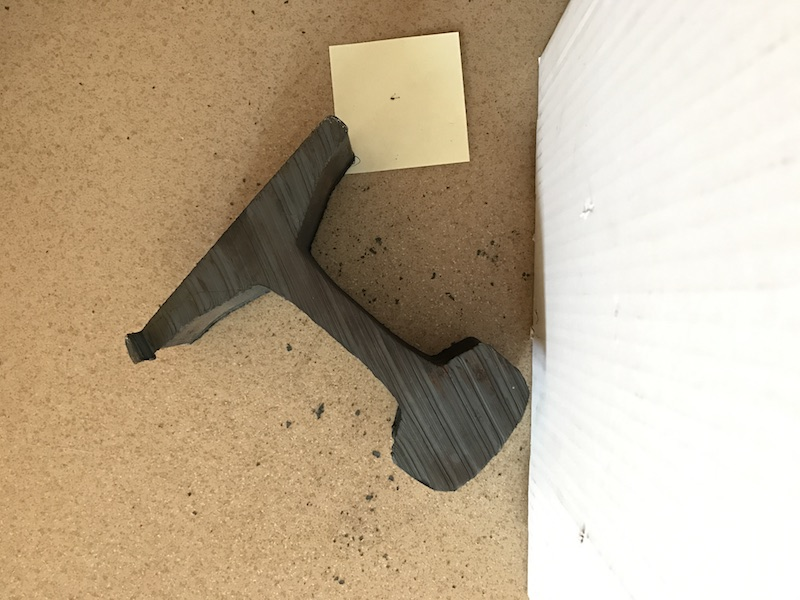
\includegraphics[width=0.75\textwidth]{images/example_splint}
	\caption{An example of a splint}
	\label{fig:example_of_a_splint}
\end{figure}

\paragraph{}
Figure \ref{fig:pattern_to_code} shows a zoomed in part of the splint with aforementioned lines pattern and a corresponding code.
\begin{figure}[H]
     \centering
     \subfloat[Zoomed in pattern]{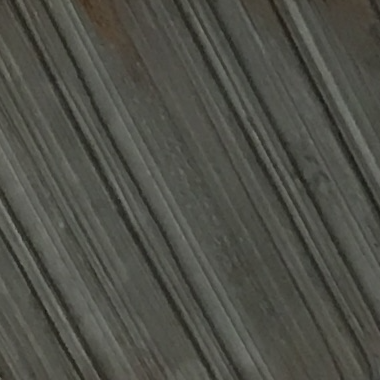
\includegraphics[width=0.4\textwidth]{images/example_pattern_closeup}}
     \hfill
     \subfloat[Corresponding code]{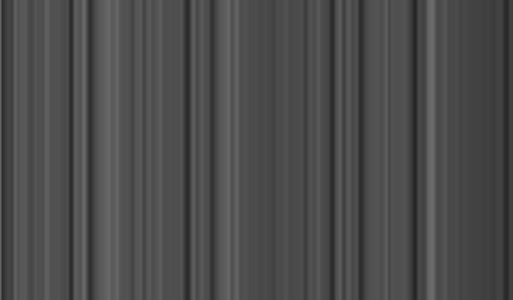
\includegraphics[width=0.4\textwidth]{images/example_pattern_to_code}}
     \caption{A zoomed-in pattern and a corresponding code}
     \label{fig:pattern_to_code}
\end{figure}

\paragraph{}
The code from the patter in figure \ref{fig:pattern_to_code} was computed simply by averaging the grayscale value of pixels along the lines and then reading those values from left to right on a line perpendicular to the lines of the pattern.

\begin{figure}[H]
     \centering
     \subfloat[A regular barcode]{
\includegraphics[width=0.4\textwidth]{images/example_barcode}}
     \hfill
     \subfloat[Pattern code]{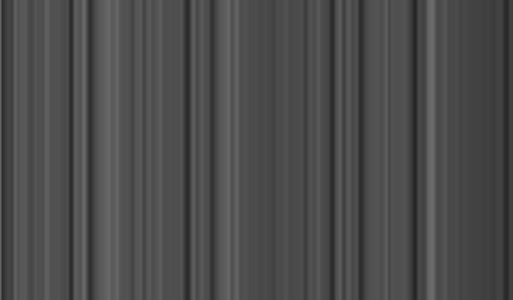
\includegraphics[width=0.4\textwidth]{images/example_pattern_to_code}}
     \caption{Comparison of a regular barcode with pattern code}
     \label{fig:regular_vs_pattern_code}
\end{figure}
\paragraph{}
After the code is found we need a way to compare them. It cannot simply be direct comparison, but rather defining some metric of similarity and if the output is above some threshold value we will say, that the codes are equal.

\chapter{State of the Art}
\paragraph{}
Here I'll write about some other solutions that are already on the market

\chapter{System's Architecture}
\section{The idea of the system}
The system is designed to take two images of rails and output the comparison result - a boolean value, true meaning it is the same object, false meaning the opposite. In order to obtain a photo of the rail a camera is used, that captures the alignment of the lines on the surface of the split, then that image is being passed to the program that performs the recognition and comparison process.
\begin{figure}[h]
	\centering
	
\includegraphics[width=\textwidth]{images/deployment_diagram}
	\caption{The idea of the system}
\end{figure}

\section{Image Acquisition}
\paragraph{}
Images used while developing the program were shot on a regular iPhone. Also the light conditions were far from ideal. Plenty of images contain either light reflexes or extensive shades. Moreover, image background and surroundings differ, which makes the processing even more error prone (see figure \ref{fig:different_lightning_conditions}).

\begin{figure}[H]
     \centering
     \subfloat[]{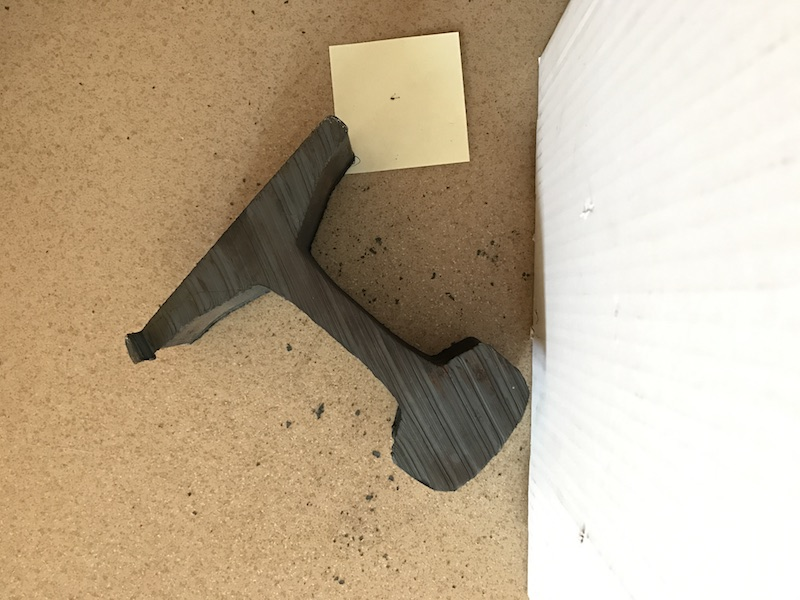
\includegraphics[width=0.45\textwidth]{images/example_rail}}
     \qquad
     \subfloat[]{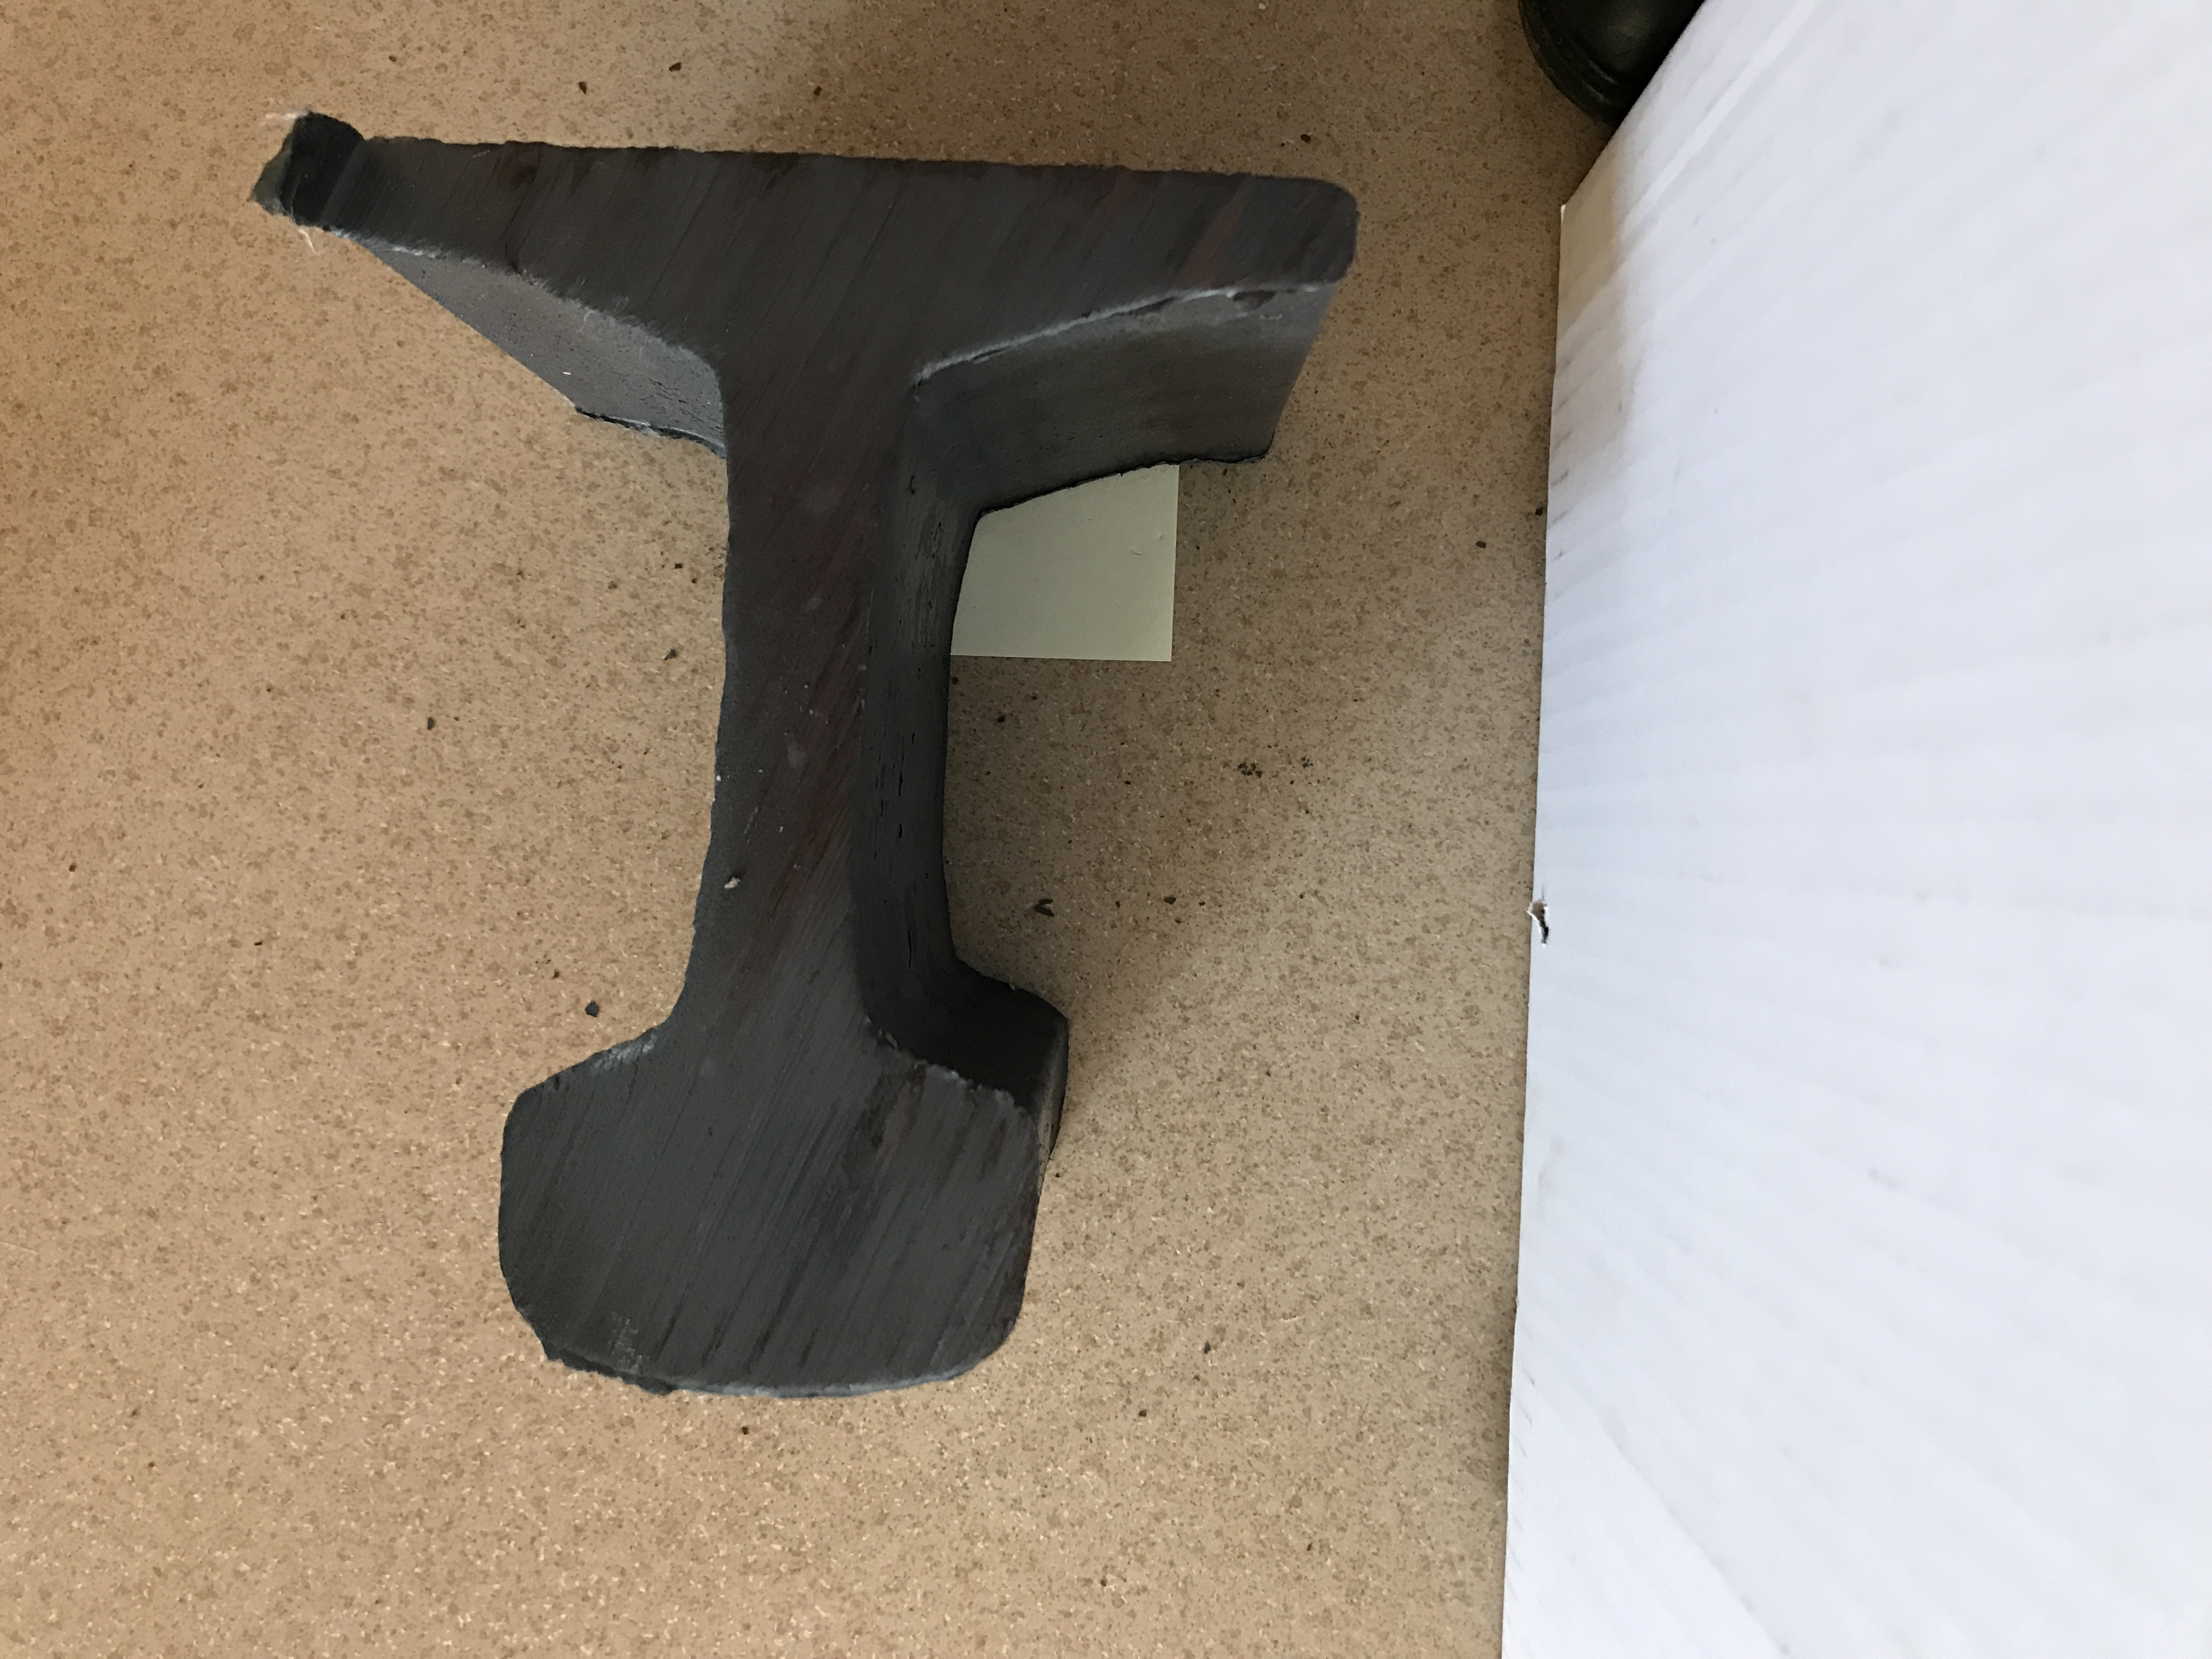
\includegraphics[width=0.45\textwidth]{images/example_rail_2}}
     \qquad
     \vfill
     \subfloat[]{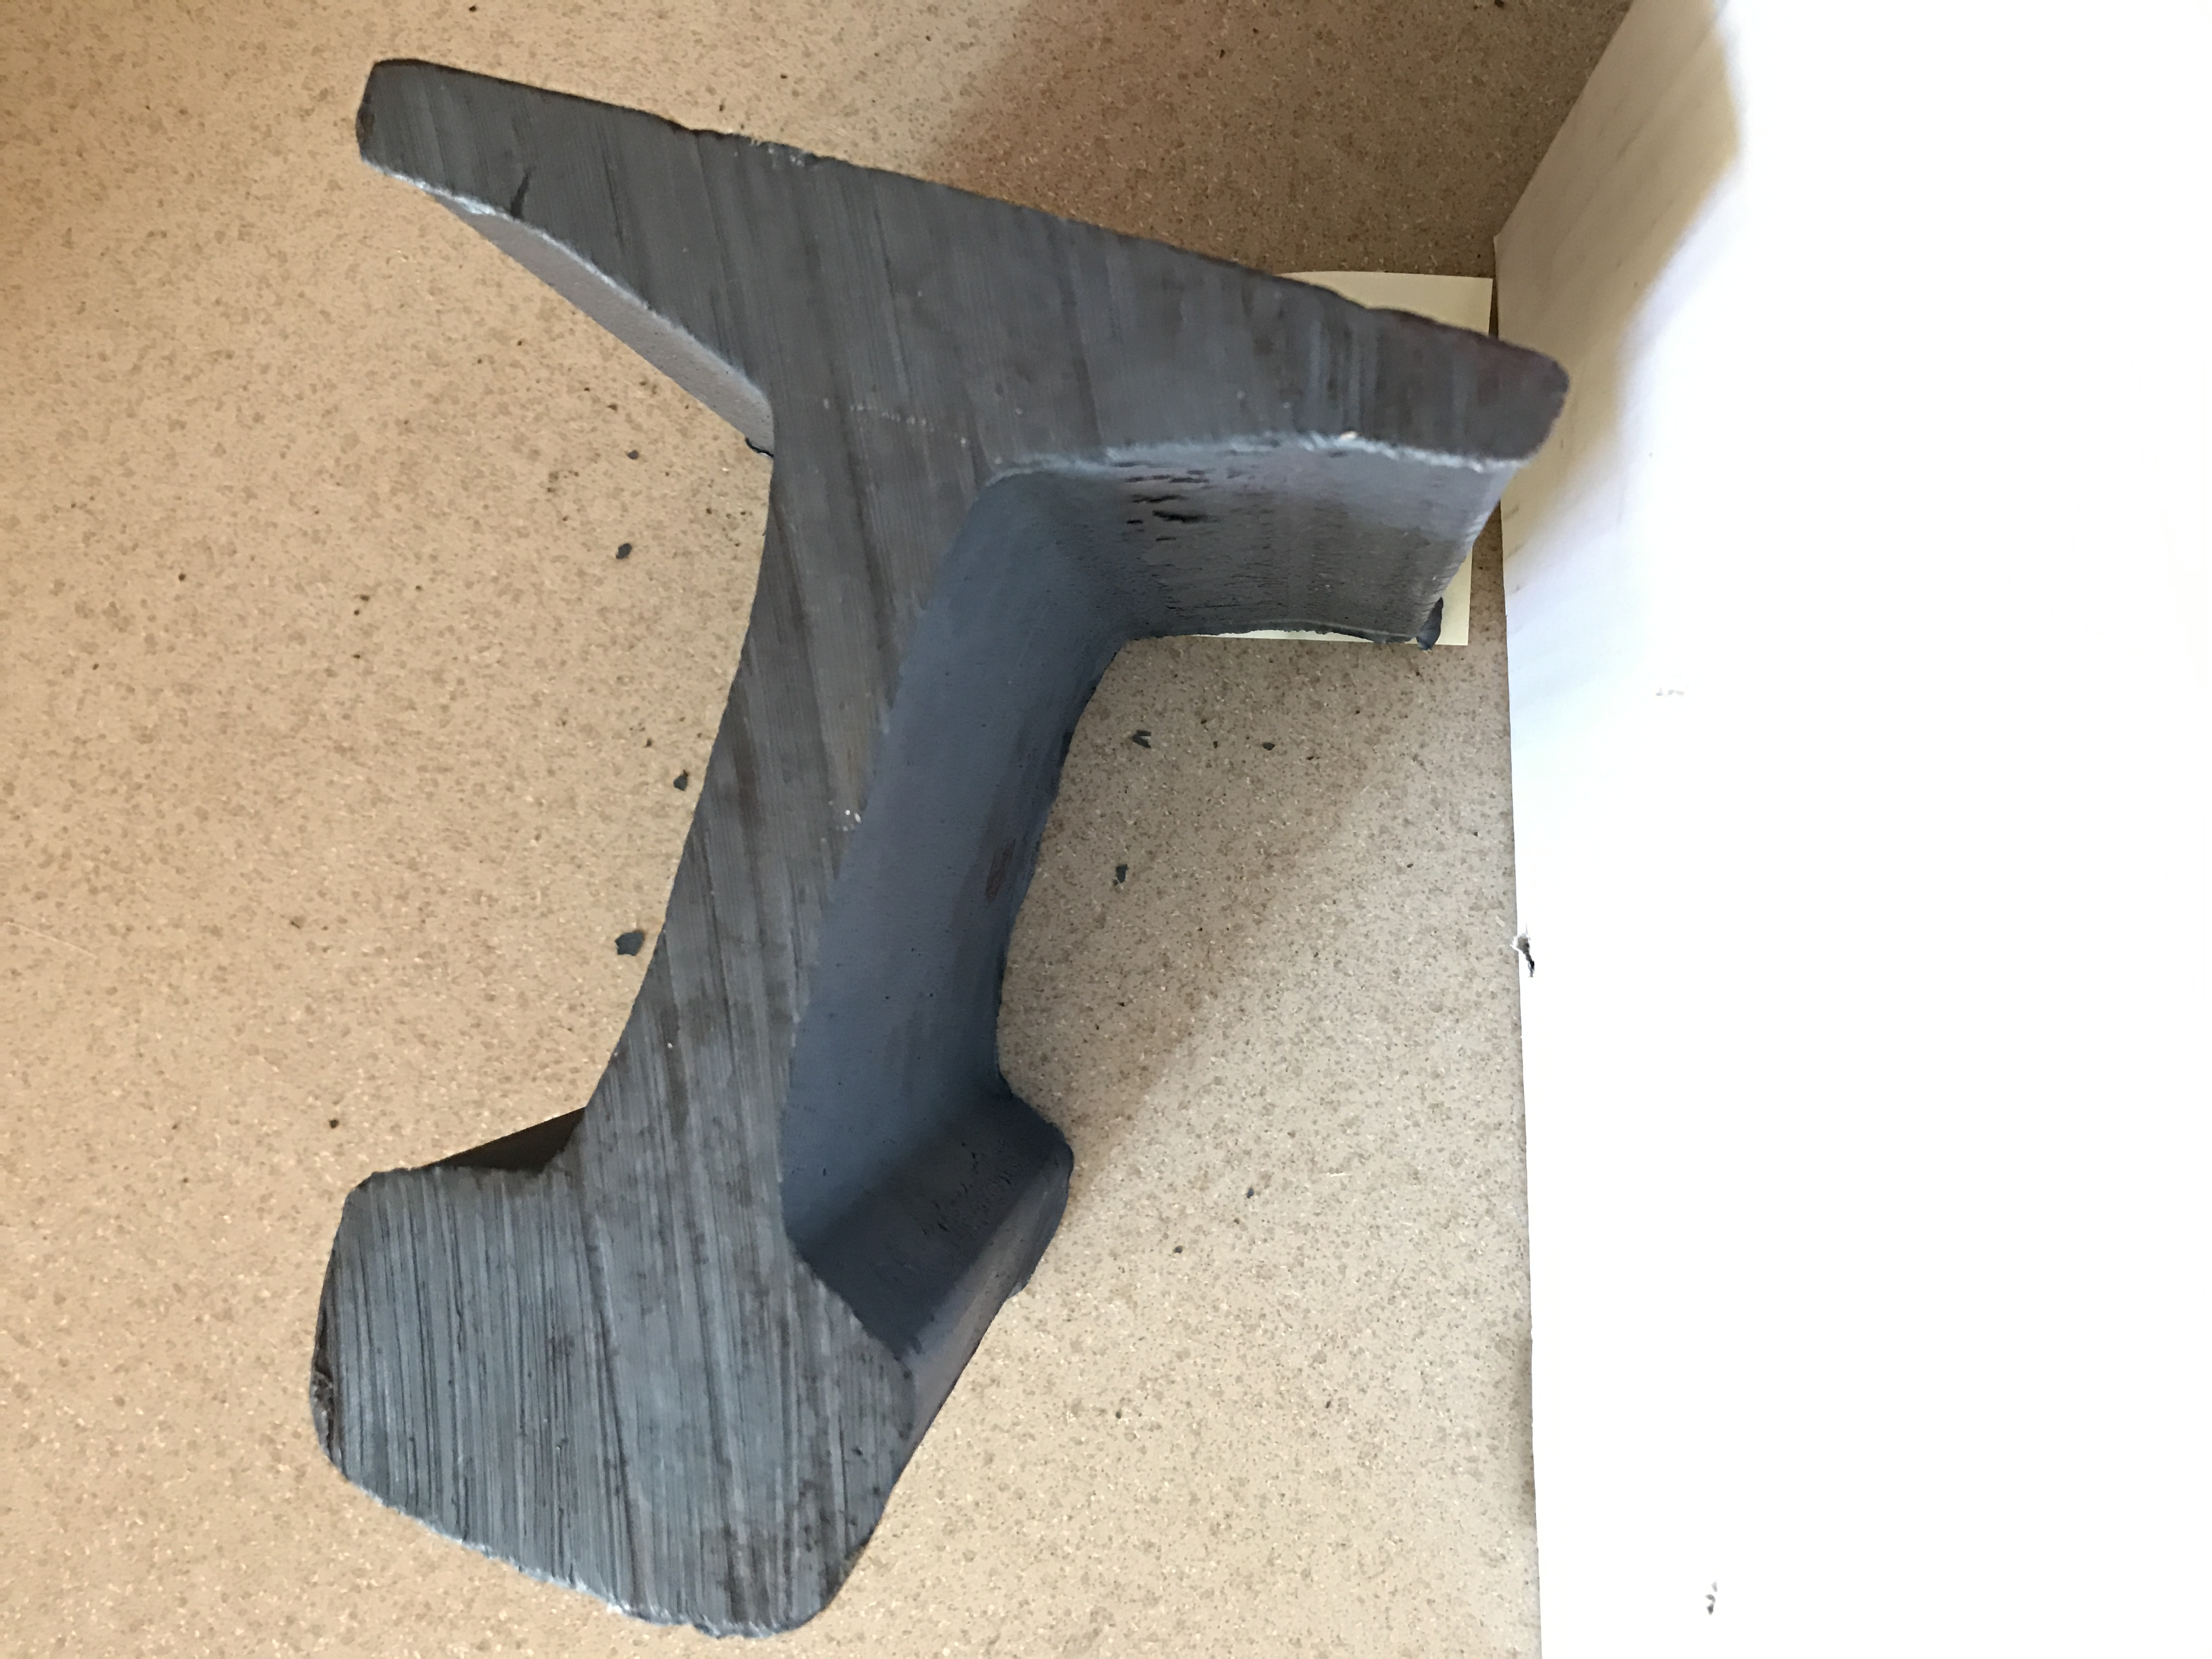
\includegraphics[width=0.45\textwidth]{images/example_rail_3}}
     \qquad
     \subfloat[]{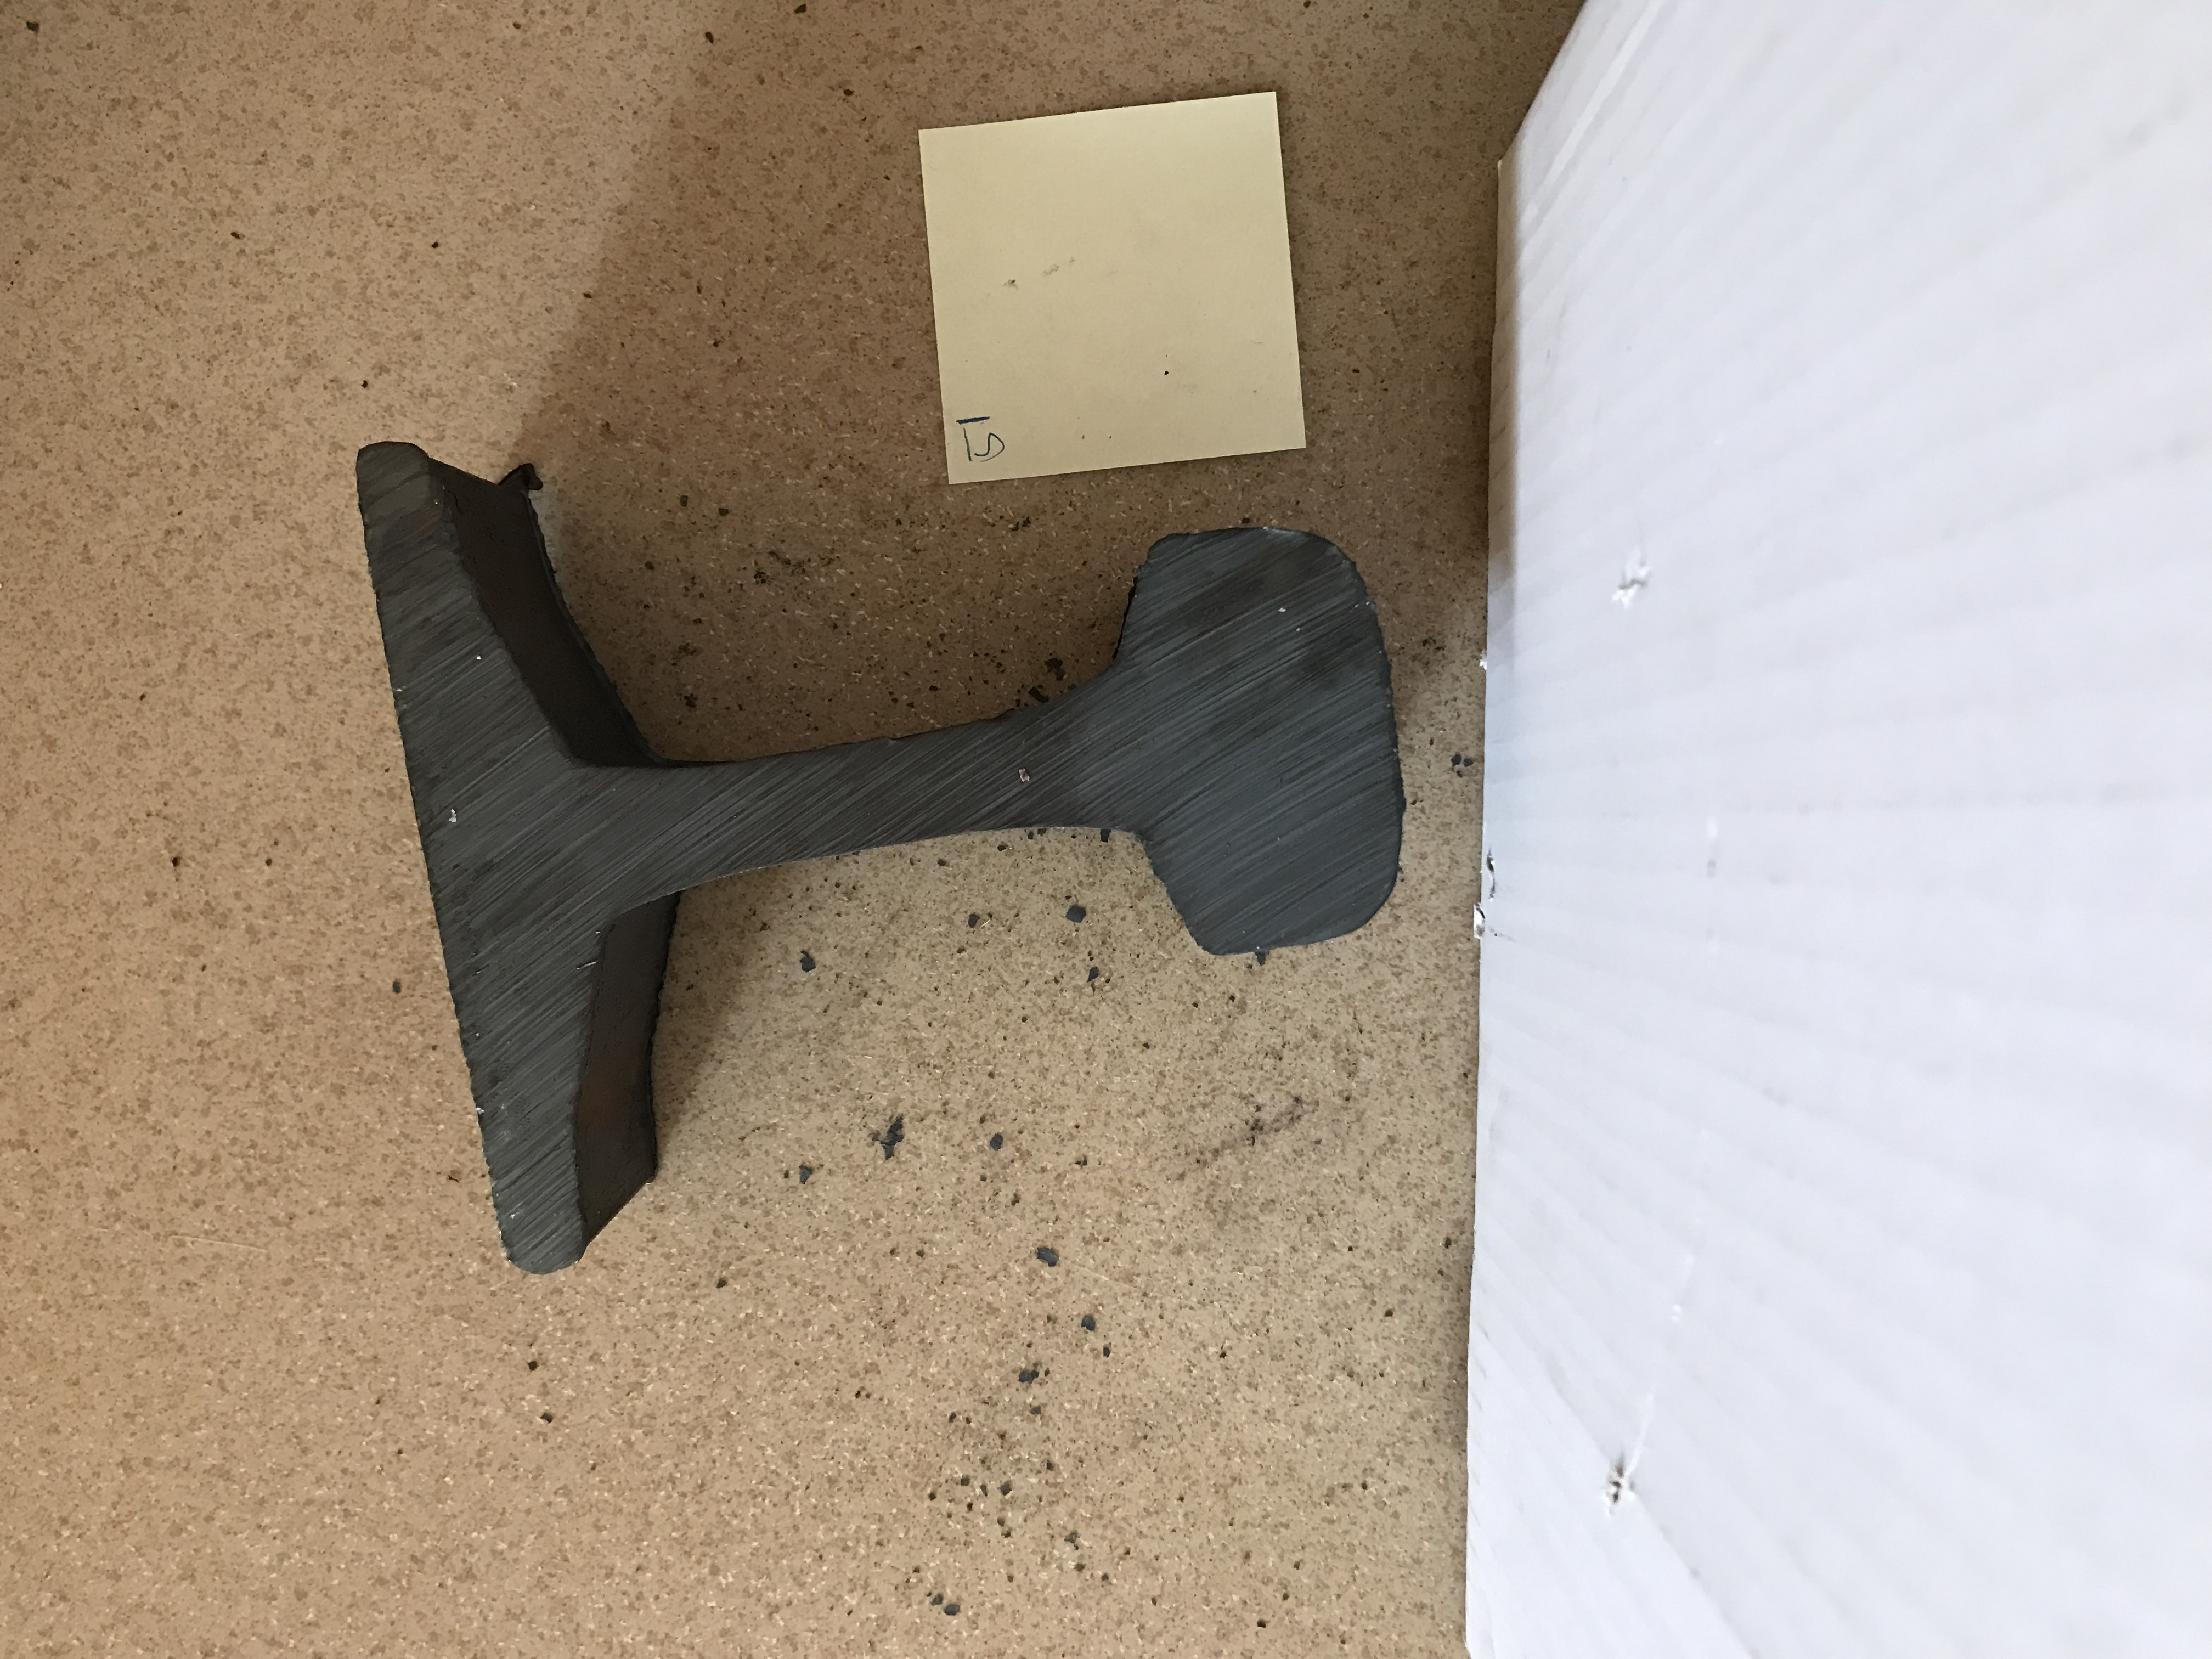
\includegraphics[width=0.45\textwidth]{images/example_rail_4}}
     \caption{Sample images of rails}
     \label{fig:different_lightning_conditions}
\end{figure}
 
\paragraph{}
However, provided the system will be implemented in production use, professional equipment will be installed (for example high quality camera) and maximal effort will be undertaken to ensure similar light conditions and background (ideally striking, monochromatic colour)

\section{Image Preprocessing}
\paragraph{Note}
The preprocessing of the image, in our case, means extracting from the input image just the parts that we are interested in and dropping all the rest. Specifically, the only part of the rail that is of interest to us is the surface. Thus the desired output of this phase is an image containing only the surface of the rail with everything else as mono-coloured background (for example white). Since this aspect is not the main focus of this thesis, only a simplified, although giving very promising results, approach will be shown. It is likely that fine-tuning the proposed algorithm would lead to having a fully working preprocessing stage.

\paragraph{Initial algorithm}
Before computing the "barcode" representation of the rail, there is a couple of steps required to enable processing. The primary goal is extraction of the split's shape from the image, effectively ignoring everything else. Let us now look at the first attempt to approach this task using following techniques:

\begin{enumerate}
	\item Image thresholding (binary) - it is a function that for a given grayscale pixel\footnote{For color input, following RGB to grayscale transformation is used: \begin{equation*}Y \gets 0.299 * R + 0.587 * G + 0.114 * B\end{equation*}For more details please consult \autoref{sec:image_thresholding}} assigns one of two values {A, B}. A is assigned to all of the pixels with value greater than some threshold value and B otherwise.
	$$
	threshold (pixel, T) = \begin{cases}
		A, pixel.value > T \\
		B, pixel.value <= T
	\end{cases}
	$$
	\item Finding contours - a function finding curves joining continuous points, having same colour or intensity
\end{enumerate}

\begin{algorithm}
	\begin{spacing}{1.5}
	\begin{algorithmic}[1]
		\Function{extract}{$grayscale$}
			\State $threshold \gets \textbf{cv2.threshold}(grayscale)$
			\State $contours \gets \textbf{cv2.findContours}(threshold)$
			\State $railContour \gets \textbf{maxArea}(contours)$
			\State $mask \gets \textbf{createMask}(railContour)$
			\State \textbf{return} $\textbf{cropImage}(grayscale, mask)$
		\EndFunction
	\end{algorithmic}
	\end{spacing}
	\caption{Extracting the shape of the split - first approach}
	\label{alg:extract_shape_1st}
\end{algorithm}

\paragraph{}
The algorithm \ref{alg:extract_shape_1st} greatly simplifies the usage of OpenCV library - Open Source Computer Vision Library (\url{https://opencv.org/}), for which an overview is provided in \autoref{sec:opencv}. It does not provide any of the other required parameters for library functions and it also discards other return values. Function steps provide just the essential parts of the algorithm to present the idea. In line 2, a thresholding operation is applied to distinguish foreground and background on the image. Line 3, for previously obtained binary input, detects contours. Then, in line 4, a contour with maximal area is selected, from which a mask is created in line 5. That mask is then used, in line 6, to cut the foreground from the original input image. Please find high-level information about used functions:

\begin{enumerate}
	\item \textbf{maxArea()} - finds the contour with maximal area amongst ones provided as the parameter
	\item \textbf{createMask()} - creates a mask that includes the whole shape of contour (i.e. the edge and the interior) for a given contour
	\item \textbf{cropImage()} - to a given image applies a given mask, effectively cutting out just those pixels specified by the mask 
\end{enumerate}

\paragraph{}
The \textbf{cv2.} prefix in selected functions from algorithm \ref{alg:extract_shape_1st} indicates that they come from second version of Python bindings for OpenCV. Please find excerpt from OpenCV documentation attached: \cite{opencv-docs}

\begin{enumerate}
	\item \textit{retval, dst} = \textbf{threshold}(\textit{src, thresh, maxval, type[, dst]}) - Applies a fixed-level threshold to each array element. The function returns the computed threshold value. \small{\begin{itemize}
		\item \textit{src} - input array
		\item \textit{thresh} - threshold value
		\item \textit{maxval} - max value to use with the binary and binary inverse type
		\item \textit{type} - thresholding type
		\item \textit{dst} - output array
	\end{itemize}}
	\item \textit{image, contours, hierarchy} = \textbf{findContours}(\textit{image, mode, method[, contours[, hierarchy[, offset]]]}) - Finds contours in a binary image \small{\begin{itemize}
		\item \textit{image} - source, an 8-bit single-channel image
		\item \textit{mode} - contour retrieval mode
		\item \textit{method} - contour approximation method
		\item \textit{contours} - detected contours
		\item \textit{hierarchy} - optional vector with information about the image topology
		\item \textit{offset} - optional offset by which every contour point is shifted
	\end{itemize}}
\end{enumerate}

\paragraph{Improved algorithm}
Further development of the preprocessing algorithm led to a little bit more complex series of steps presented in algorithm \ref{alg:extract_shape_2nd}. Instead of converting whole RGB image to grayscale, the multi-channel array is split into separate single-channel arrays. Empirical experiments showed that for the given set of input images best results can be obtained when using just the red colour channel. The thresholding phase is now executed with threshold value computed from the histogram (first, peak value that corresponds to the rail is found and then, after performing simple algebraic operations, it is used to obtain the value). The thresholding process returns a binary image where white colour denotes area that is most likely a part of the rail and a black colour otherwise. Such a binary image then undergoes a series of corresponding image blurring (using median blur filter) and morphological opening (which is a series of erosions followed by dilations). To complete the process and fill some gaps that may have appeared in some of the previous phases, a fill holes procedure is applied.

\begin{algorithm}
	\begin{spacing}{1.5}
	\begin{algorithmic}[1]
		\Function{extract}{$image$}
			\State $redChannel \gets$ R channel from the $image$
			\State $railPeak \gets$ rail peak from histogram of $redChannel$
			\State $threshold \gets \textbf{threshold}(redChannel, railPeak)$
			\State $blur \gets \textbf{cv2.medianBlur}(threshold)$
			\For{$i \gets 0\ \textbf{to}\ repetitions$}
				\State $opening \gets \textbf{open}(blur)$
				\State $blur \gets \textbf{cv2.medianBlur}(opening)$
			\EndFor
			\State $filled \gets \textbf{fillHoles}(blur)$
			\State $contours \gets \textbf{cv2.findContours}(filled)$
			\State $railContour \gets \textbf{maxArea}(contours)$
			\State $mask \gets \textbf{createMask}(railContour)$
			\State \textbf{return} $\textbf{cropImage}(grayscale, mask)$
		\EndFunction
	\end{algorithmic}
	\end{spacing}
	\caption{Extracting the shape of the split - improved approach}
	\label{alg:extract_shape_2nd}
\end{algorithm}

\paragraph{}
Let us now look at the Algorithm \ref{alg:extract_shape_2nd}. In line 2, red channel is taken from the input image. Next, in line 3, a thresholding value is selected as the most-frequently occurring red value and is used in line 4 to perform the actual threshold. In line number 5 a blurring operation is applied to the binary output of thresholding. The loop in lines 6 to 9 performs repetitive opening and blurring of the binary image. After the loop finishes, any holes that might have occurred, are treated as foreground, in line 10. Lines 11-14 repeat last steps from previous algorithm \ref{alg:extract_shape_1st}.

\paragraph{}
Please find excerpt from OpenCV documentation, for function from algorithm \ref{alg:extract_shape_2nd}, attached: \cite{opencv-docs}

\begin{enumerate}
	\item \textit{dst} = \textbf{medianBlur}(\textit{src, ksize[, dst]}) - Blurs an image using the median filter. \small{\begin{itemize}
		\item \textit{src} - input
		\item \textit{dst} - destination array of the same size and type as src
		\item \textit{ksize} - aperture linear size; it must be odd and greater than 1
	\end{itemize}}
\end{enumerate}

\begin{figure}[H]
     \centering
     \subfloat[Before]{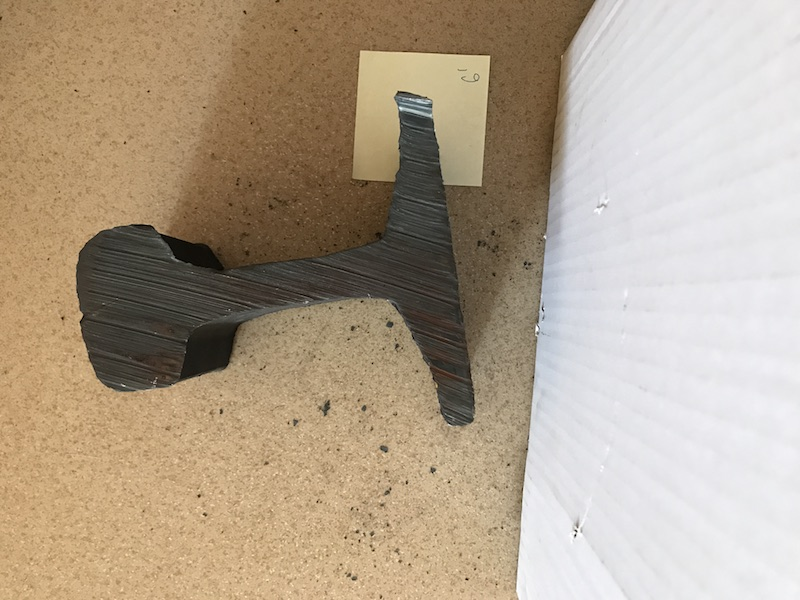
\includegraphics[width=0.45\textwidth]{images/good_before_preprocessing}}
     \qquad
     \subfloat[After thresholding]{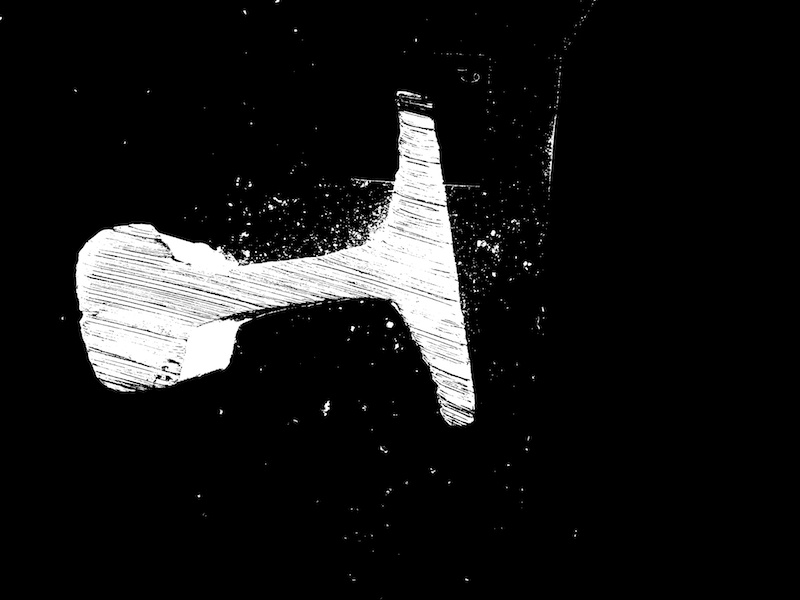
\includegraphics[width=0.45\textwidth]{images/good_after_thresholding}}
     \qquad
     \vfill
     \subfloat[After opening and blurring]{
\includegraphics[width=0.45\textwidth]{images/good_after_opening_and_blurring}}
     \qquad
     \subfloat[Shape detected]{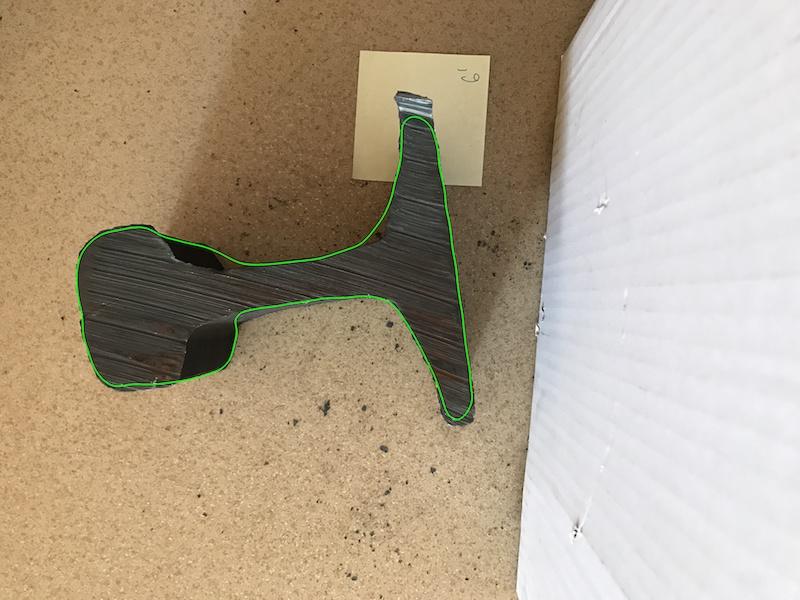
\includegraphics[width=0.45\textwidth]{images/good_after_preprocessing}}
     \caption{Stages of preprocessing - successful}
     \label{fig:preprocessing}
\end{figure}

\section{Image Processing}
\paragraph{}
Given that the main purpose of the thesis is the identification of foundry details, we can skip further contemplation of the preprocessing phase. The shape detection and extraction can be treated as a separate algorithm that needs to be developed and fine-tuned.

\paragraph{}
Assuming we have such an algorithm and thus a successful preprocessing phase, in the actual computing phase the input images contain only the surfaces of the rails (see figure \ref{fig:preprocessing_outputs}).

\paragraph{Note}
The actual input images for performing tests of the processing phase, as shown in figure \ref{fig:preprocessing_outputs}, were prepared manually. It was done using free and open source image editor GIMP (\url{https://www.gimp.org/}), by utilizing its' \textit{Free Select Tool}.

\begin{figure}[H]
     \centering
     \subfloat[]{\fbox{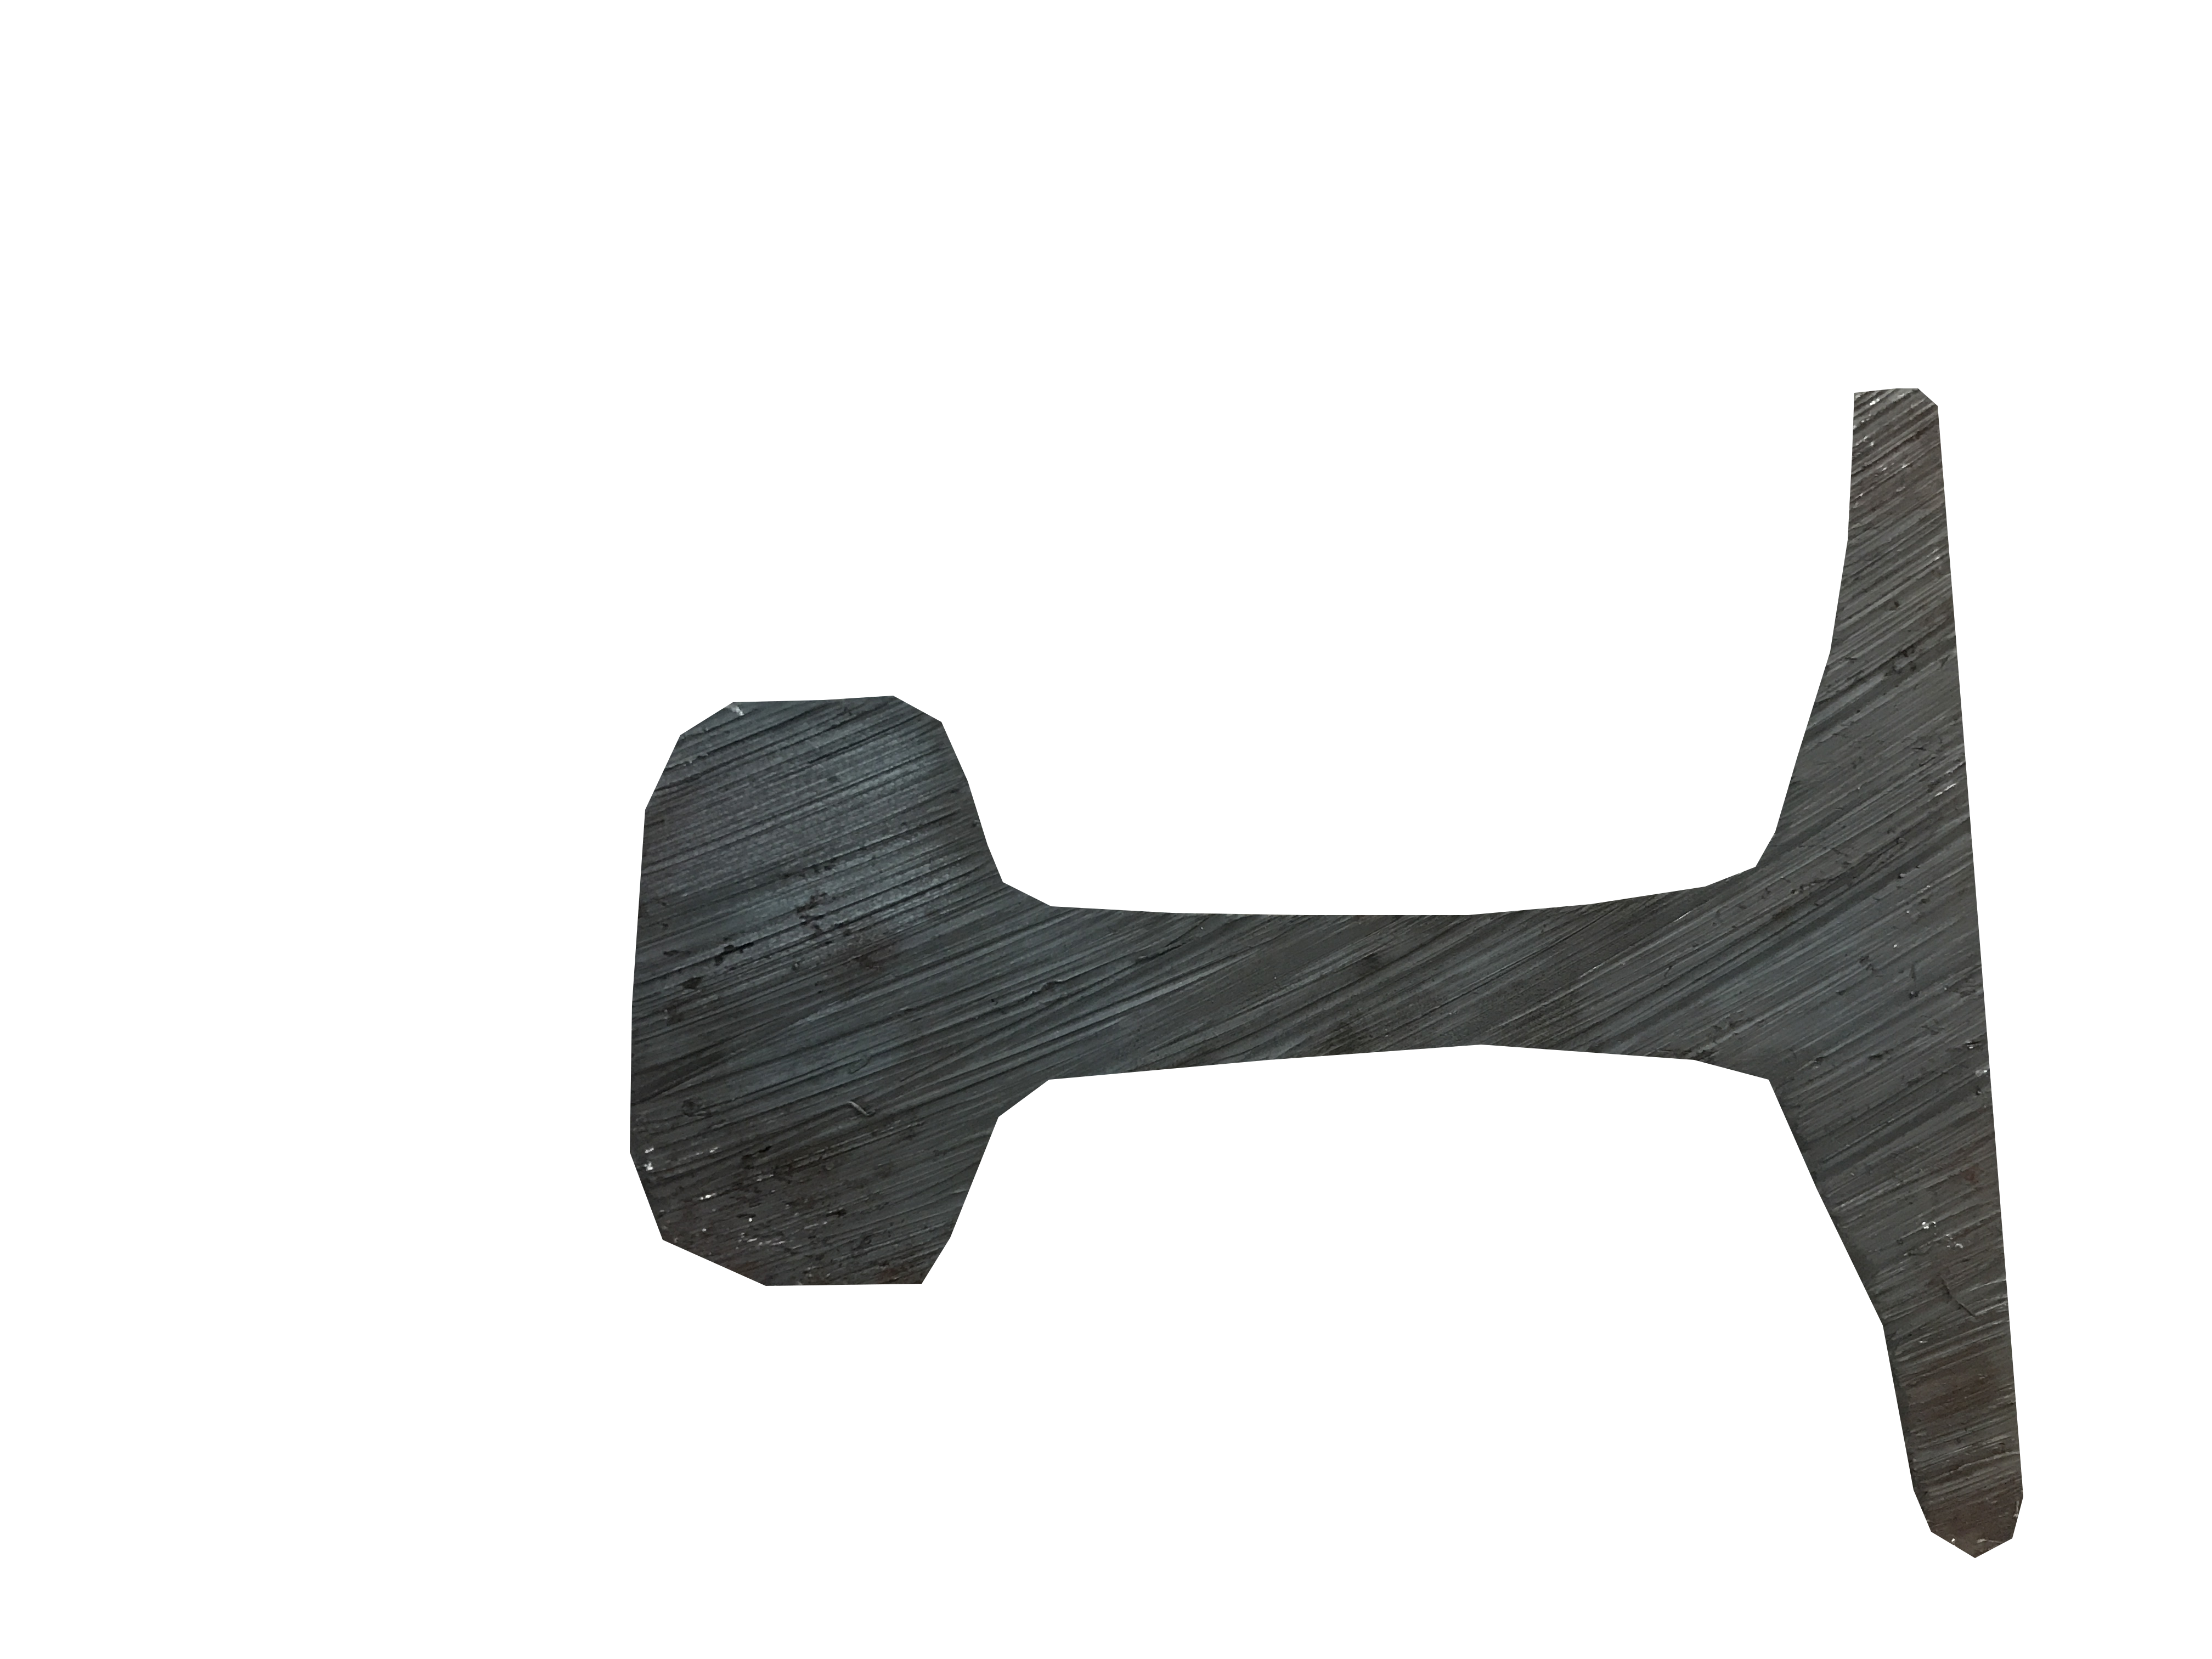
\includegraphics[width=0.45\textwidth]{images/preprocessed_1}}}
     \qquad
     \subfloat[]{\fbox{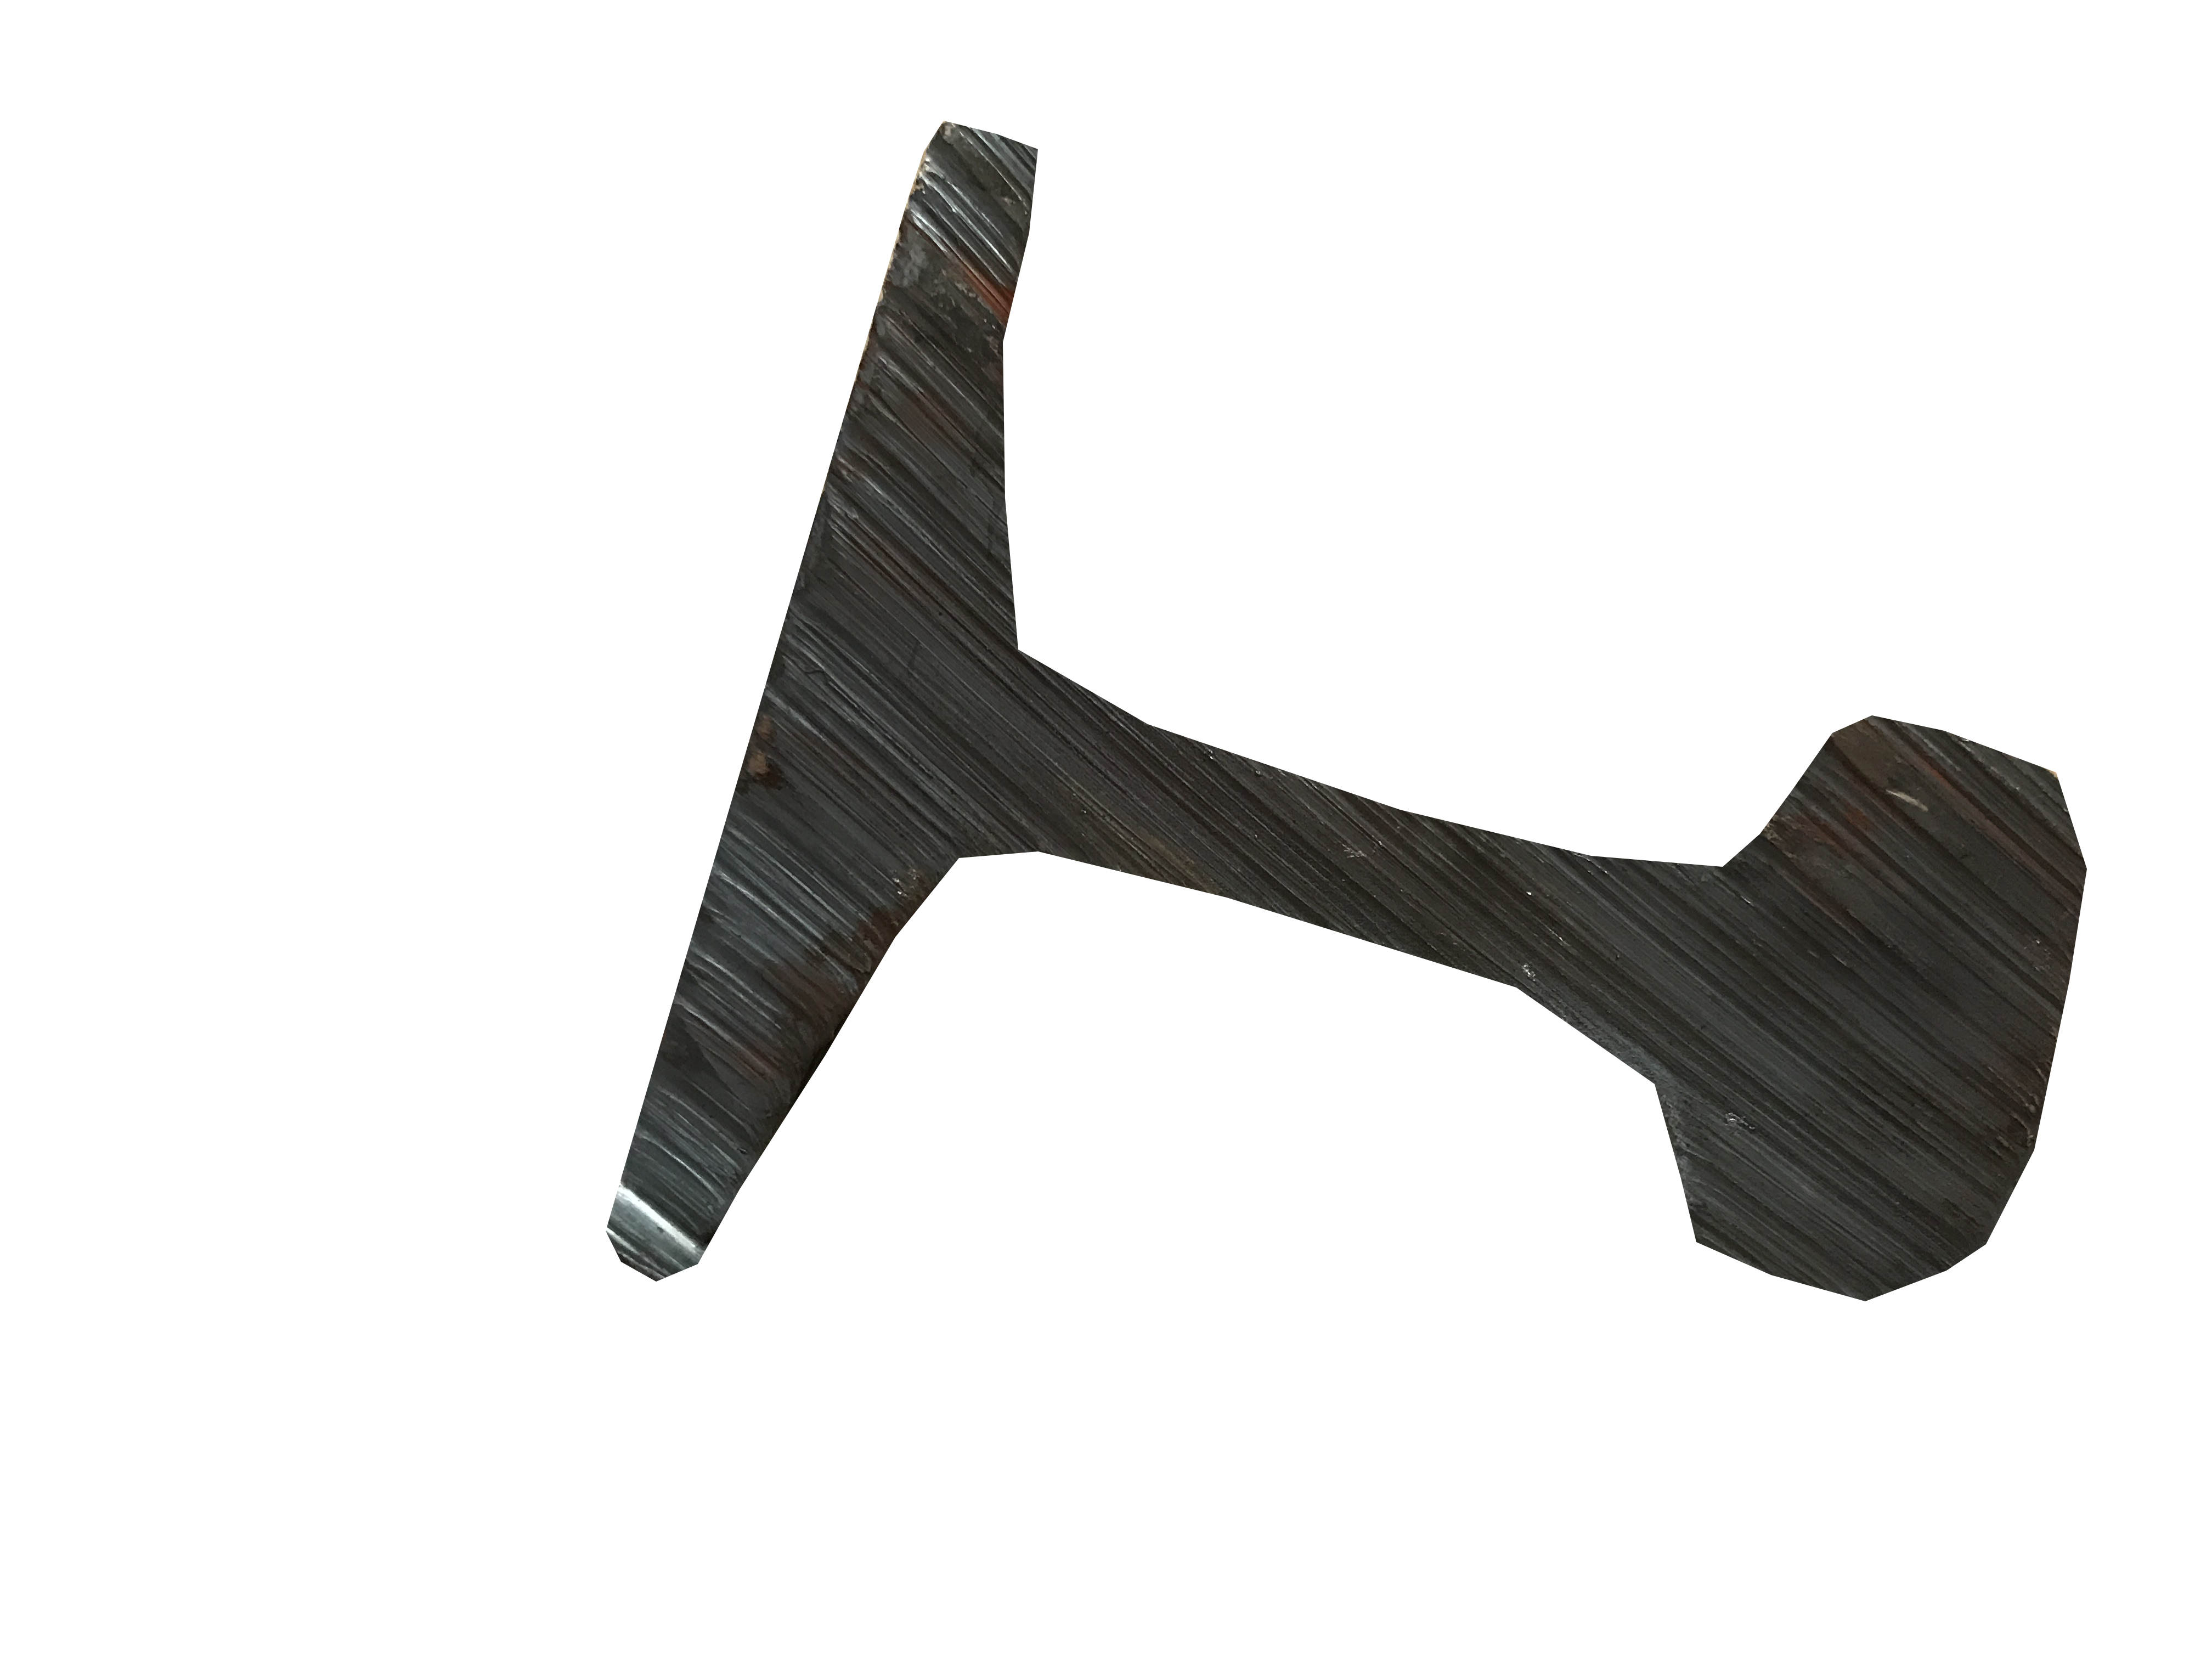
\includegraphics[width=0.45\textwidth]{images/preprocessed_2}}}
     \qquad
     \vfill
     \subfloat[]{\fbox{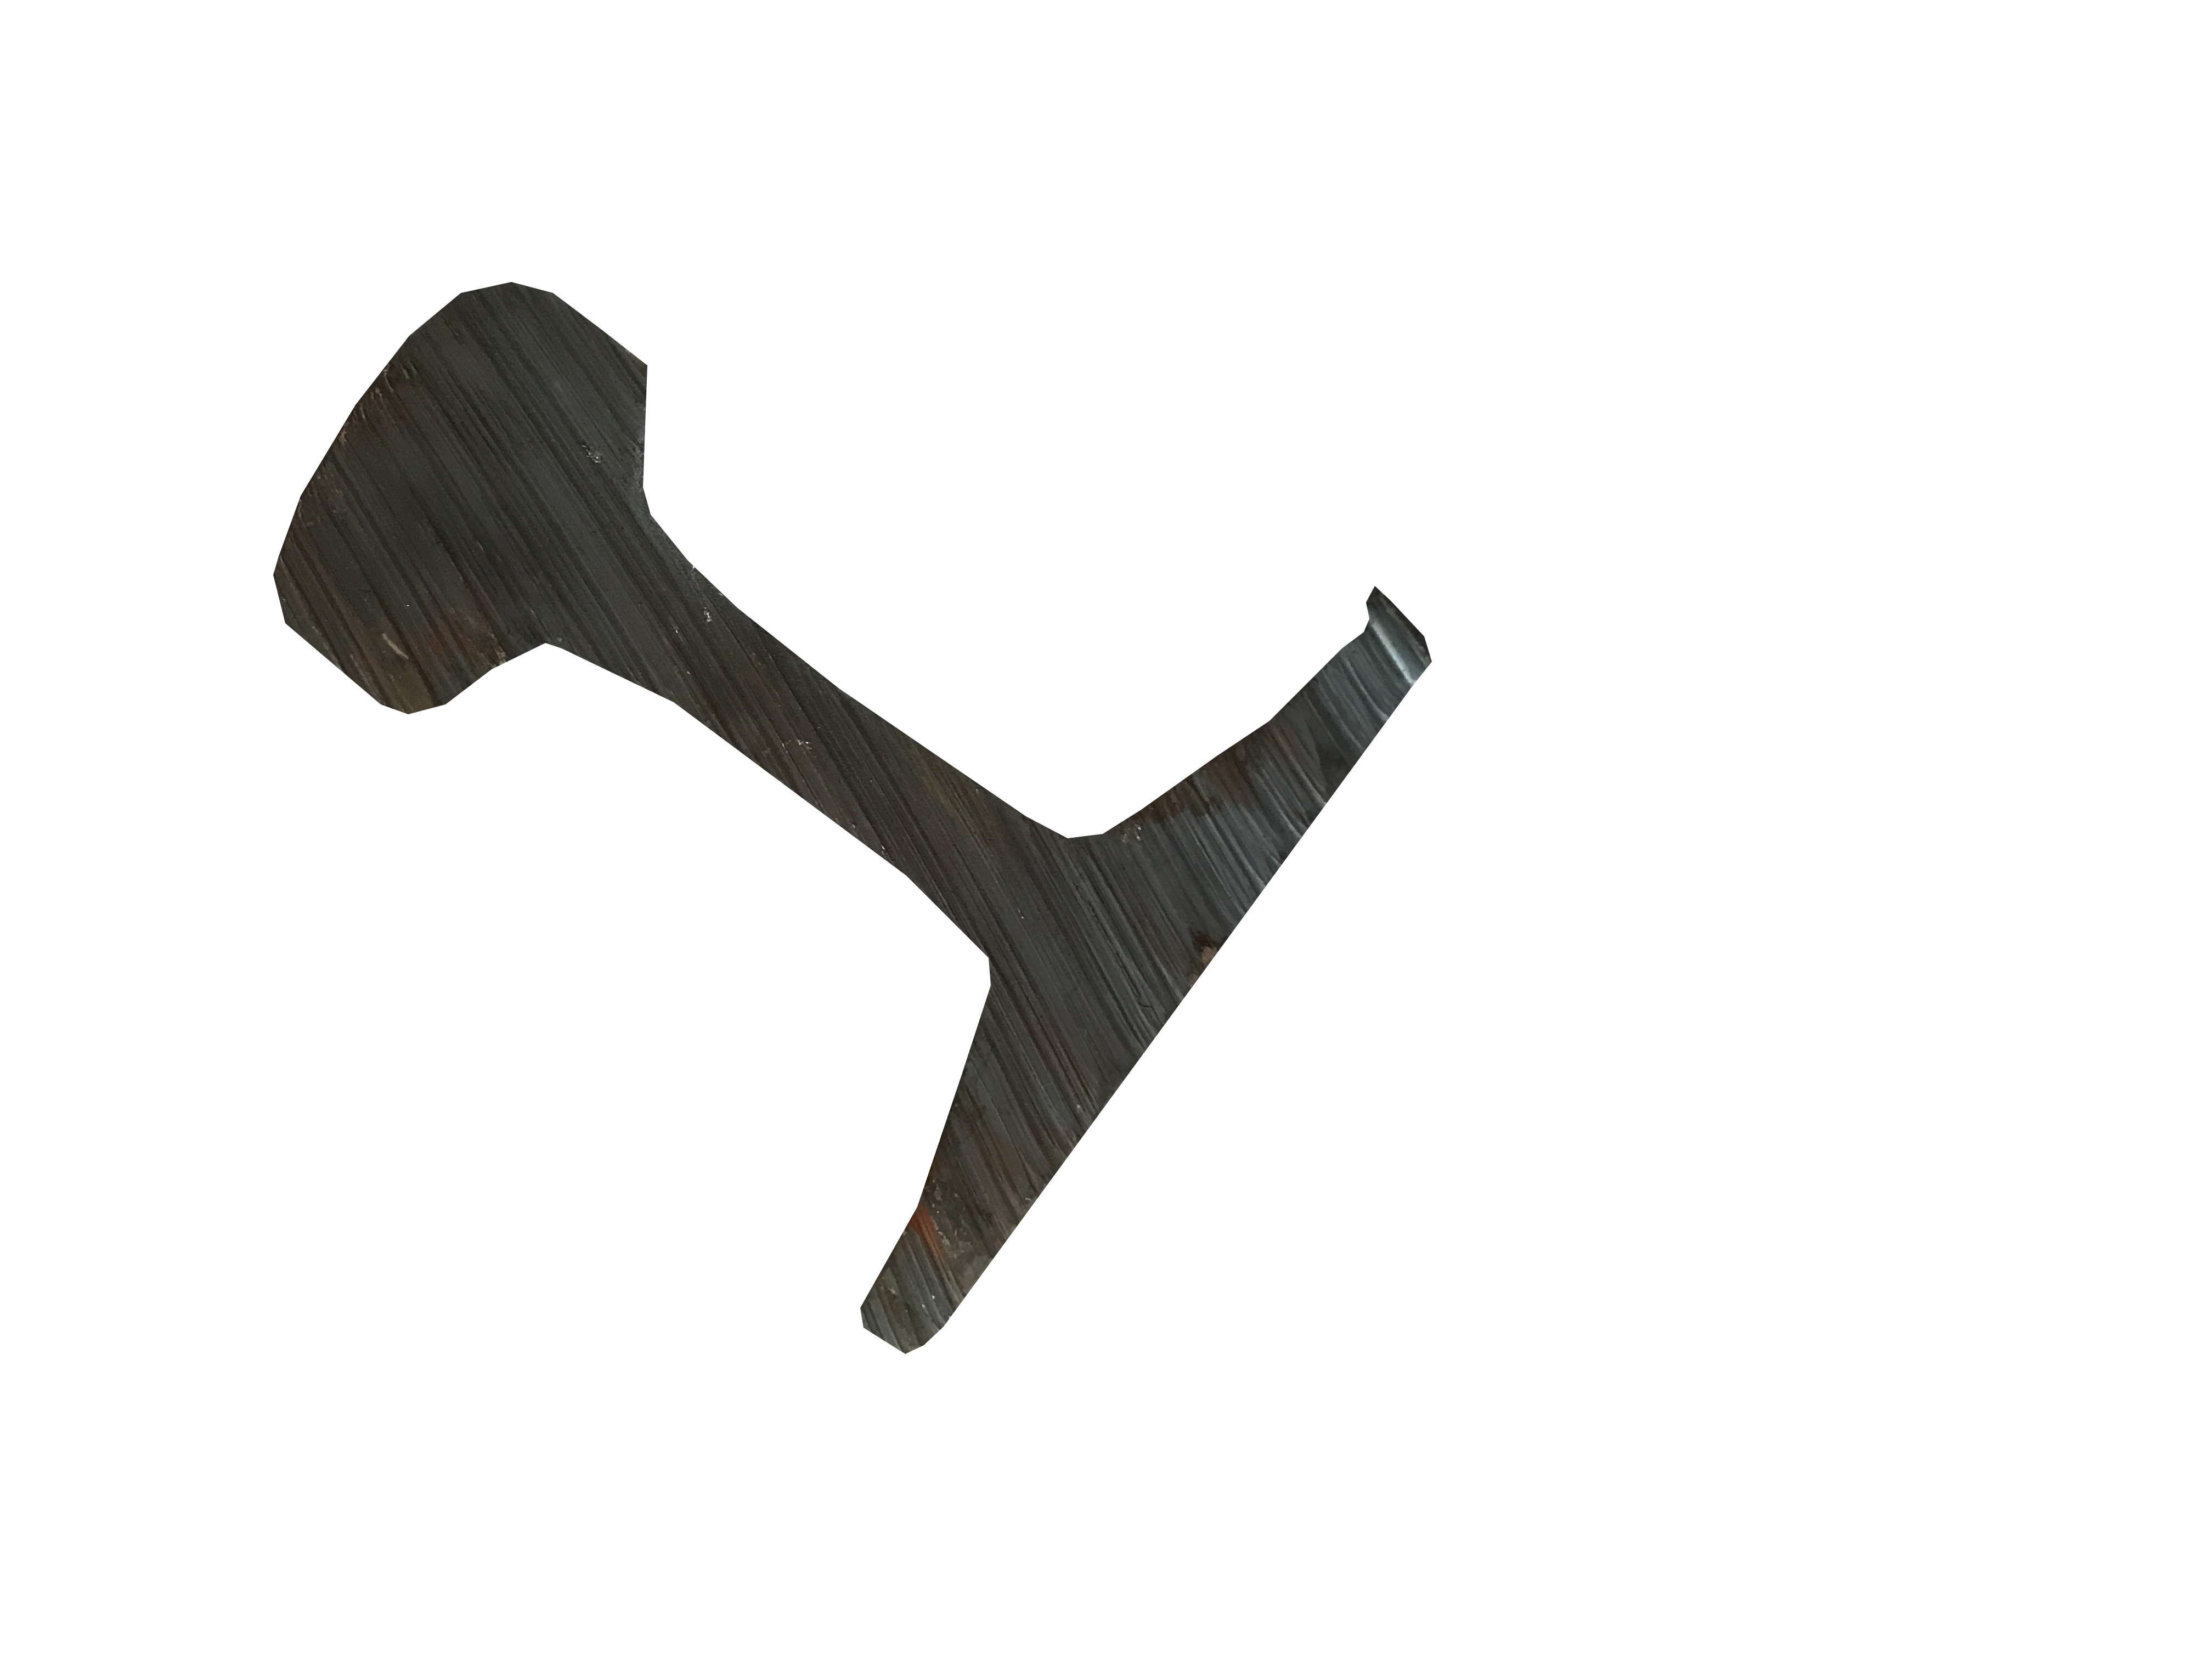
\includegraphics[width=0.45\textwidth]{images/preprocessed_3}}}
     \qquad
     \subfloat[]{\fbox{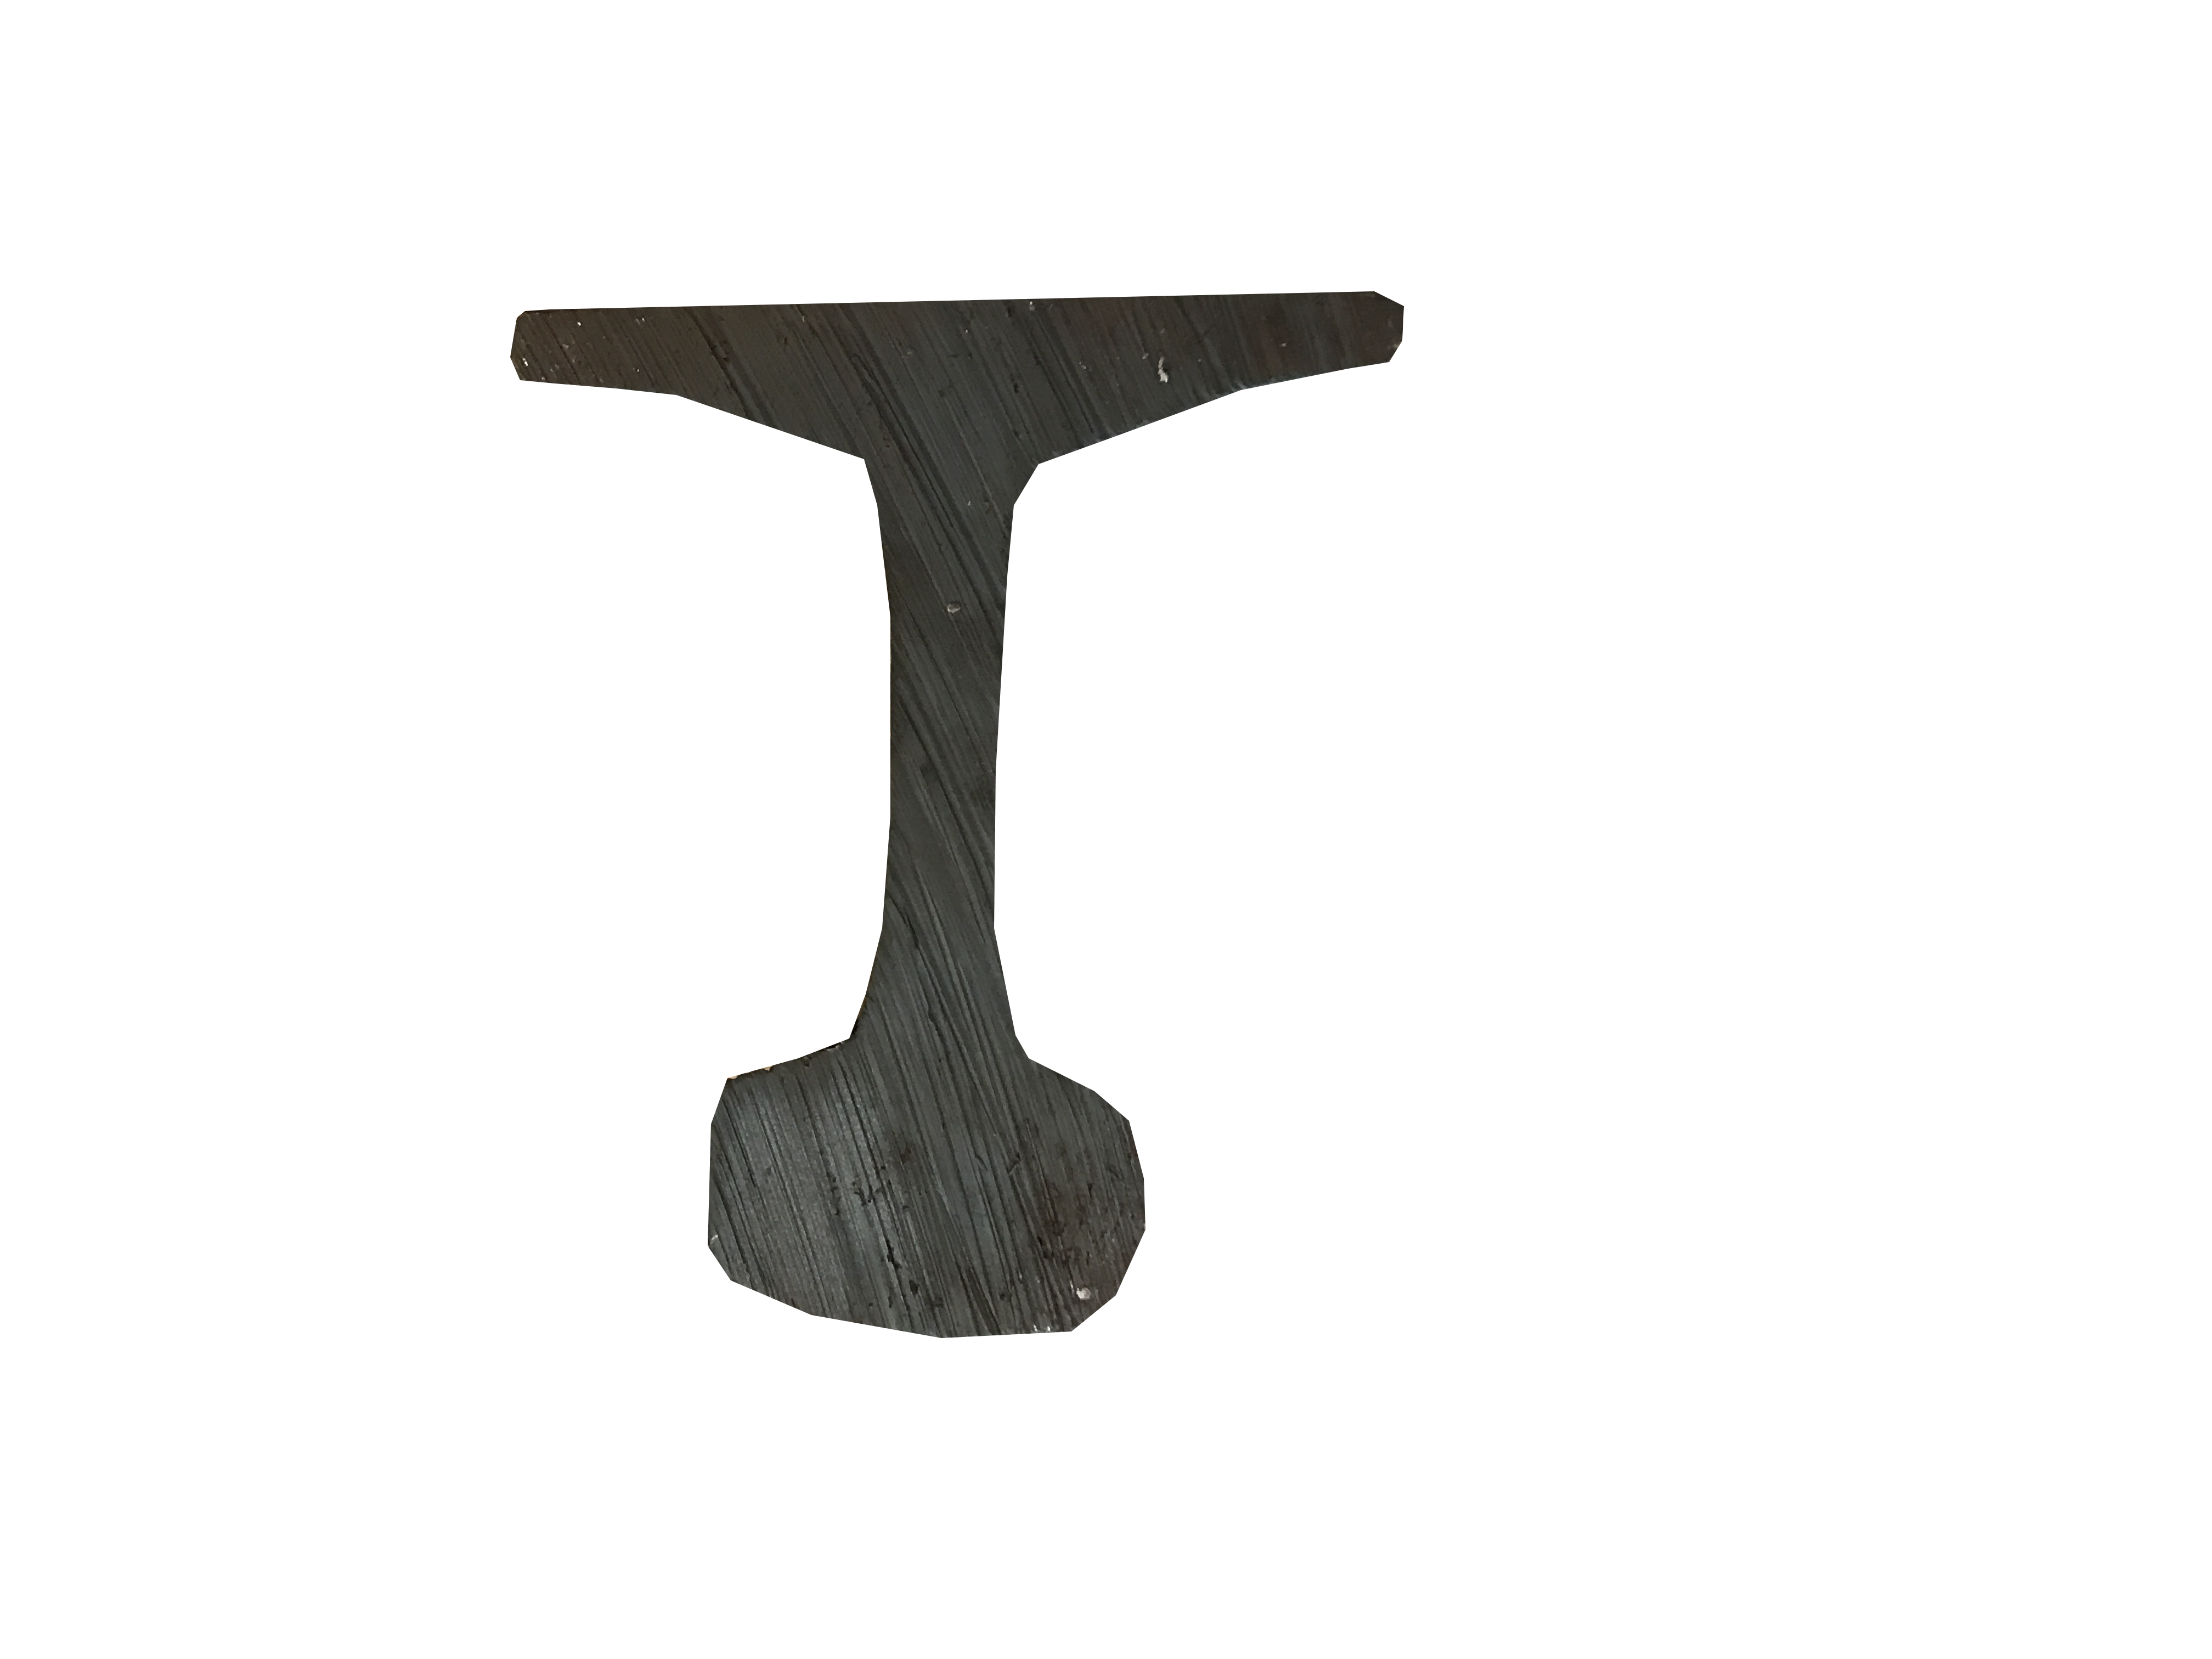
\includegraphics[width=0.45\textwidth]{images/preprocessed_4}}}
     \caption{Preprocessing outputs}
     \label{fig:preprocessing_outputs}
\end{figure}

\paragraph{}
In order to reduce complexity of the processing phase, a need to find some optimizations emerged. One of the solutions that was under investigation was to scale the image down - but it led to more noise being introduced and thus the comparison results being less accurate. Experiments and development of the processing algorithm showed that the most significant part for the comparison of barcodes lies in the upper half of the rail surface - the "ellipse-shaped" part of it. It is due to the fact that this area is the most stable across all of the images in terms of the barcode readability and consistency. This is why the lower part of the image is actually dropped altogether from the analysis.

\paragraph{}
Let us now look at the Algorithm \ref{alg:comparing} for comparing two images. Lines 2 and 3 are responsible for taking just the upper half of both input images. Next, in lines 4 and 5, dominant angles for both upper halves are found. The conditional expression in lines 6-9 detects a difference in dominant angles higher than the admissible threshold and immediately signals that the two images show different rails if this threshold is crossed. In lines 9 and 10 both upper halves are rotated so that the barcode is perpendicular to the X-axis. In line 11 a function is called to find the maximal comparison result of the two rotated images. It performs also slight rotations to accommodate for some minor differences in detected dominant angles. Finally, in line 12, the returned result is verified and if it is satisfactory, then we assume the original input images show the same rail. Otherwise, the output is negative. 

\begin{algorithm}
	\begin{spacing}{1.5}
	\begin{algorithmic}[1]
		\Function{compare}{$image1, image2$}
			\State $image1\_up \gets$ upper half from the $image1$
			\State $image2\_up \gets$ upper half from the $image2$
			
			\State $angle1 \gets \textbf{dominantAngle}(image1\_up)$
			\State $angle2 \gets \textbf{dominantAngle}(image2\_up)$
			
			\If{$\textbf{abs}(angle1 - angle2) > \textbf{THRESHOLD\_ANGLE}$}
				\State \textbf{return} FALSE
			\EndIf
			
			\State $rotated1 \gets \textbf{rotate}(image1\_up, angle1)$
			\State $rotated2 \gets \textbf{rotate}(image2\_up, angle2)$
			
			\State $result \gets \textbf{findMaxComparisonResult}(rotated1, rotated2)$
			\State \textbf{return} $result > \textbf{THRESHOLD\_COMPARISON}$
		\EndFunction
	\end{algorithmic}
	\end{spacing}
	\caption{Comparing two preprocessed rail images}
	\label{alg:comparing}
\end{algorithm}

\begin{itemize}
	\item \textbf{dominantAngle(image)} - this function finds the most frequent angle amongst the lines that create the pattern. The image first undergoes Canny Edge detection, so line detection algorithm can later be used. It does so by utilising OpenCV's \textbf{HoughLinesP}\footnote{It works similar to the standard Hough line transformation, that is described in \autoref{sec:hough_lines} with two important differences. The lines are represented as start and end points. The second difference is the ability to specify the minimum length of a line segment and the separation between collinear segments required for the algorithm not to join them into a single longer segment.\cite{learning-opencv-3}} function from which those angles can be computed, rounded and the dominant one is selected. The pseudocode and some explanation for this algorithm is provided later in this chapter. (See algorithm \ref{alg:dominant_angle})
	\item \textbf{rotate(image, angle)} - this function simply rotates the image by a given angle. It is used to point the lines that form the pattern perpendicular to X-axis.
	\item \textbf{findMaxComparisonResult(image1, image2)} - this function is returning the final comparison result. In order to alleviate some differences in the dominant angle resulting in slightly different rotations, this function itself also does minor rotations for first of the images and each such rotation is being compared with the second image. Maximum value of those comparisons is then returned as the final value.
\end{itemize}

\paragraph{}
Algorithm \ref{alg:dominant_angle} detects the most-frequently occurring angle among the lines on the rail's surface. In line 2 the light is equalized, then, in line 3, a color space conversion to grayscale is applied. Such an image is passed to Canny function for edge detection in line 4. Next an accumulator array for detected angles is created in line 5 and, in line 6, probabilistic Hough lines transform is applied to the detected edges. The loop in lines 7 through 12, for each line that was reported from the Hough transform, computes the slope angle and adds it to the accumulator. In line 13, a histogram of the angles is created, and the dominant one is chosen in lines 14 and 15.

\begin{algorithm}
	\begin{spacing}{1.5}
	\begin{algorithmic}[1]
		\Function{dominantAngle}{$color\_image$}
			\State $equalized \gets \textbf{equalizeLight}(color\_image)$
			\State $gray \gets \textbf{cv2.cvtColor}(equalized)$
			\State $edges \gets \textbf{cv2.Canny}(gray)$
			\State $angles \gets []$
			\State $lines \gets \textbf{cv2.HoughLinesP}(edges)$
			\For{$line \gets lines$}
				\State $x1, y1, x2, y2 \gets line$
				\State $a \gets $ slope of $x1, y1, x2, y2$
				\State $angle \gets$ get angle for $slope$
				\State $angles.append(angle)$
			\EndFor
			\State $histogram \gets \textbf{np.histogram}(angles, bins=360, range=(0, 180))$
			\State $convolution \gets \textbf{np.convolve}(hist, \textbf{np.ones}(6))$
			\State \textbf{return} $\textbf{np.argmax}(convolution) / 2.0$
		\EndFunction
	\end{algorithmic}
	\end{spacing}
	\caption{Finding the dominant angle}
	\label{alg:dominant_angle}
\end{algorithm}

\paragraph{}
Please find excerpt from OpenCV documentation, for functions from algorithm \ref{alg:dominant_angle}, attached: \cite{opencv-docs}

\begin{enumerate}
	\item \textit{dst} = \textbf{cvtColor}(\textit{src, code[, dst[, dstCn]]}) - Converts an image from one color space to another. \small{\begin{itemize}
		\item \textit{src} - input image
		\item \textit{dst} - output image of the same size and depth as src
		\item \textit{code} - color space conversion code
		\item \textit{dstCn} - number of channels in the destination image
	\end{itemize}}
	\item \textit{edges} = \textbf{Canny}(\textit{image, threshold1, threshold2[, edges[, apertureSize[, L2gradient]]]}) - Finds edges in an image using the Canny algorithm. \small{\begin{itemize}
		\item \textit{image} - source, an 8-bit single-channel image
		\item \textit{edges} - output edge map
		\item \textit{threshold1} - first threshold for the hysteresis procedure
		\item \textit{threshold2} - second threshold for the hysteresis procedure
		\item \textit{apertureSize} - aperture size for the Sobel operator
		\item \textit{L2gradient} - a flag, indicating whether a more accurate $L_2$ norm
	\end{itemize}}
	\item \textit{lines} = \textbf{HoughLinesP}(\textit{image, rho, theta, threshold[, lines[, minLineLength[, maxLineGap]]]}) - Finds line segments in a binary image using the probabilistic Hough transform. \small{\begin{itemize}
		\item \textit{image} - source, an 8-bit single-channel image
		\item \textit{lines} - output vector of lines
		\item \textit{rho} - distance resolution of the accumulator in pixels
		\item \textit{theta} - angle resolution of the accumulator in radians
		\item \textit{threshold} - accumulator threshold parameter
		\item \textit{minLineLength} - min line length
		\item \textit{maxLineGap} - max allowed gap between points on the same line to link them	
	\end{itemize}}
\end{enumerate}

\paragraph{}
In order to accommodate for some relic peaks, it is actually not the most frequently occurring angle but it is accumulatively taken within 3 degrees and only then the max is picked.

\begin{figure}[H]
     \centering
     \subfloat[Original input]{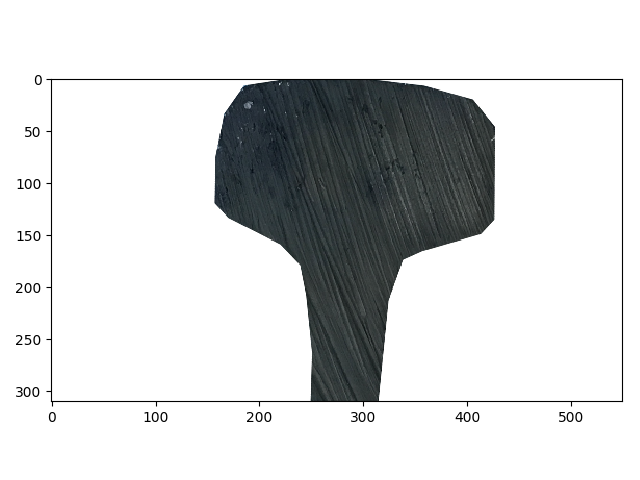
\includegraphics[width=0.75\textwidth]{images/up}}
     \vfill
     \subfloat[Rotated]{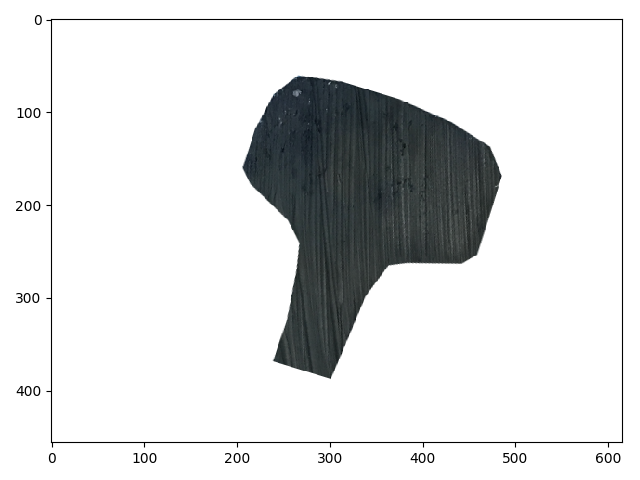
\includegraphics[width=0.75\textwidth]{images/rotated_up}}
     \caption{Rotation perpendicular to X-axis}
     \label{fig:image_rotation}
\end{figure}

\begin{figure}[H]
     \centering
     \subfloat[Pattern code]{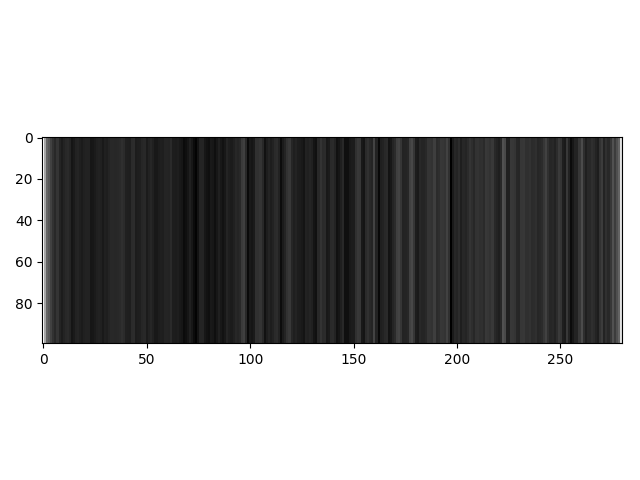
\includegraphics[width=0.75\textwidth]{images/rotated_up_code}}
     \vfill
     \subfloat[Corresponding histogram]{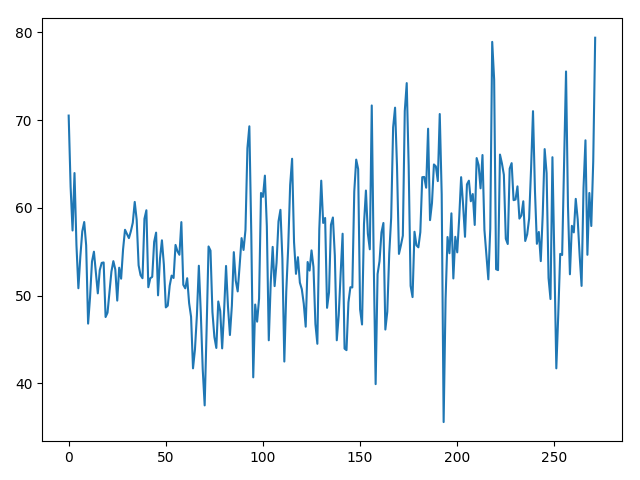
\includegraphics[width=0.75\textwidth]{images/rotated_up_hist}}
     \caption{Code and its' histogram}
     \label{fig:code_with_histogram}
\end{figure}

\paragraph{}
Figure \ref{fig:image_rotation} presents the already-extracted upper half of the rail surface before and after the rotation. This procedure outputs an image, where the "barcode" lines are aligned perpendicular to the X-axis. 

\paragraph{}
Next, figure \ref{fig:code_with_histogram} shows the code that was read from the image (it actually is a single-row vector, only for plotting purposes that row is multiplied and we can see the code) and the histogram that corresponds to its grayscale values.

\paragraph{}
The whole process of mapping the rail image to a barcode (single-row vector) was to reduce the dimensionality of the task on hand. Now it was just a matter of finding a smart way to compare this vectors and assign them some similarity score. This is where the histogram that was computed on the earlier stages comes in handy. There are already known methods of comparing them and one that was performing well was chosen in the comparison algorithm implementation.

\paragraph{}
In order to actually compare two histograms $H$ (equation \ref{eq:hist_H}) and $G$ (equation \ref{eq:hist_G}) with the same number of bins\footnote{$h_1$ is the number of elements in the first bin, $h_2$ in the second bin, e.t.c. The same holds true for $g_1$, $g_2$, \dots, $g_n$}:

\begin{equation}
	H = \{h_1, h_2, \dots, h_n\}
	\label{eq:hist_H}
\end{equation}

\begin{equation}
	G = \{g_1, g_2, \dots, g_n\}
	\label{eq:hist_G}
\end{equation}
a metric $d(H, G)$ is to be chosen. The algorithm uses \textbf{correlation} (which is selected by using \textbf{CV\_HISTCMP\_CORREL} flag for OpenCV's \textit{compareHist} function). The metric is then defined as:
\begin{equation}
	d(H, G) = \frac{\sum_{i=1}^{n}(h_i - \bar{h})(g_i - \bar{g})}{\sqrt{\sum_{i=1}^{n}(h_i - \bar{h})^2 \sum_{i=1}^{n}(g_i - \bar{g})^2}}
	\label{eq:hist_comparison}
\end{equation}
where:
\begin{equation}
	\bar{h} = \frac{1}{n} \sum_{i=1}^{n} h_i
\end{equation}
and:
\begin{equation}
	\bar{g} = \frac{1}{n} \sum_{i=1}^{n} g_i
\end{equation}
while $n$ being the total number of bins in histogram.

\paragraph{Example}
Let us now look at a concrete example of comparing two histograms. Suppose we have two input arrays



\begin{equation*}
	A_H = [0,0,1,1,1,1,2,2,2]
\end{equation*}

and

\begin{equation*}
	A_G = [0,0,1,1,1,2,2,2,2]
\end{equation*}

\paragraph{}
Table \ref{tab:histogram_comparison} shows count of different values in both input arrays, whereas figure \ref{fig:histogram_comparison_plot} presents plots of those histograms.

\begin{table}[H]
    \centering
	\begin{spacing}{1.5}    
    \begin{tabular}{|l|l|l|}
        \hline
        \cellcolor{gray} & \textbf{$H$} & \textbf{$G$} \\ [0.5ex]
        \hline\hline
        \textbf{0} & 2 & 2 \\ [0.5ex]
        \hline
        \textbf{1} & 4 & 3 \\ [0.5ex]
        \hline
        \textbf{2} & 3 & 4 \\ [0.5ex]
        \hline
    \end{tabular}
    \end{spacing}
    \caption{Histograms for $A_H$ ($H$) and $A_G$ ($G$)}
    \label{tab:histogram_comparison}
\end{table}

\begin{figure}[H]
     \centering
     \subfloat[]{
\includegraphics[width=0.45\textwidth]{images/histogram_1}}
     \qquad
     \subfloat[]{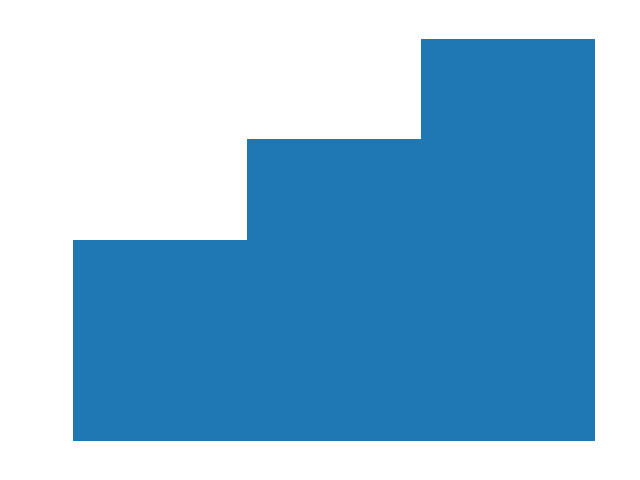
\includegraphics[width=0.45\textwidth]{images/histogram_2}}
     \caption{Plots of histograms $H$ (a) and $G$ (b)}
     \label{fig:histogram_comparison_plot}
\end{figure}

The histograms can then be represented as follows:

\begin{equation*}
	H = \{h_1, h_2, h_3\} = \{2, 4, 3\}
\end{equation*}

and:

\begin{equation*}
	G = \{g_1, g_2, g_3\} = \{2, 3, 4\}
\end{equation*}

The average values $\bar{h}$ and $\bar{g}$ can now be computed:

\begin{equation}
	\bar{h} = \frac{1}{3} * (2 + 4 + 3) = \frac{1}{3} * 9 = 3
	\label{eq:h_1_avg}
\end{equation}

\begin{equation}
	\bar{g} = \frac{1}{3} * (2 + 3 + 4) = \frac{1}{3} * 9 = 3
	\label{eq:h_2_avg}
\end{equation}

Then we should insert values from table \ref{tab:histogram_comparison} and averages from the equation \ref{eq:h_1_avg} and from the equation \ref{eq:h_2_avg} into the formula for computing the metric of histogram comparison (the equation \ref{eq:hist_comparison}):

\begin{equation}
\begin{aligned}
	d(H, G) = \frac{(2-3)*(2-3) + (4-3)*(3-3) + (3-3)*(4-3)}{\sqrt{((2-3)^2 + (4-3)^2 + (3-3)^2)((2-3)^2 + (3-3)^2 + (4-3)^2)}} = \\ \\ 
	= \frac{(-1) * (-1) + 1 * 0 + 0 * 1}{\sqrt{((-1)^2 + 1^2 + 0^2) * ((-1)^2 + 0^2 + 1^2)}} 
	= \frac{1 + 0 + 0}{\sqrt{(1+1+0)*(1+0+1)}} = \\ \\
	= \frac{1}{\sqrt{2 * 2}} = \frac{1}{\sqrt{4}} = \frac{1}{2}
	\label{eq:comparison_result}
\end{aligned}
\end{equation}

\paragraph{}
The result of histogram comparison from equation \ref{eq:comparison_result} can be confirmed with the code listing \ref{lst:comparison_result}:

\begin{lstlisting}[language=Python, caption=Histogram comparison in Python, label={lst:comparison_result},basicstyle={\ttfamily}]
import cv2
import numpy as np

a_h = np.asarray([0,0,1,1,1,1,2,2,2])
a_g = np.asarray([0,0,1,1,1,2,2,2,2])

h, _ = np.histogram(a_h, bins=3, range=(0, 2))
g, _ = np.histogram(a_g, bins=3, range=(0, 2))

d = cv2.compareHist(h, g, cv2.HISTCMP_CORREL)
\end{lstlisting}

\paragraph{}
The histograms that are obtained for two rail images may actually differ in sizes and for the aforementioned comparison method they need to be same-sized. That is why we take the shorter histogram and slide it over the longer one, do the comparison one offset at a time and take the highest from the output values.

\begin{algorithm}
	\begin{spacing}{1.5}
	\begin{algorithmic}[1]
		\Function{compareHist}{$h1, h2$}	
			\If{$\textbf{length}(h1) == \textbf{length}(h2)$}
				\State \textbf{return} $cv2.compareHist(h1, h2, cv2.HISTCMP\_CORREL)$
			\ElsIf{$\textbf{length}(h1) > \textbf{length}(h2)$}
				\State \textbf{return} $\textbf{maxHistComparison}(h1, h2)$
			\Else
				\State \textbf{return} $\textbf{maxHistComparison}(h2, h1)$
			\EndIf
		\EndFunction
	\end{algorithmic}
	\end{spacing}
	\caption{Histogram comparison}
	\label{alg:hist_comparison}
\end{algorithm}

\begin{algorithm}
	\begin{spacing}{1.5}
	\begin{algorithmic}[1]
		\Function{maxHistComparison}{$longer, shorter$}	
			\State $\text{len\_shorter} \gets \textbf{length}(shorter)$
			\State $\text{diff} \gets \textbf{length}(longer) - \textbf{length}(shorter)$
			\State $\text{max\_result} \gets -1$
			\For{$\text{offset} \gets 0\ \textbf{to}\ \text{diff}$}
				\State $\text{result} \gets \textbf{compareHist}(longer[\text{offset : offset + len\_shorter}], shorter)$
				\State $\text{max\_result} \gets \textbf{max}(\text{max\_result, result})$
			\EndFor
			\State \textbf{return} $\text{max\_result}$
		\EndFunction
	\end{algorithmic}
	\end{spacing}
	\caption{Histogram comparison - helper function}
	\label{alg:hist_comparison_helper}
\end{algorithm}

\paragraph{}
Let us now look at the algorithm \ref{alg:hist_comparison_helper}. In lines 2 and 3 the length of the shorter histogram is obtained as well as the difference in sizes between two input histograms. The variable $max\_result$ is then set to -1 to notify that no actual check was yet performed. And then the loop, in lines 5 through 8, performs histogram comparison with increasing offset on the longer histogram and assigns to $max\_result$ the maximum of the actual $max\_result$ and the new comparison result. Finally, in line 9 the overall maximum result is returned.

\paragraph{}
The final result of the comparison, as already mentioned before, takes into consideration some slight differences in the dominant angle detection (does so be applying artificial rotations in the process) and also for the size of the code (because the smaller one is searched through the larger one). Such a result - the similarity score - is then simply compared to a threshold value. If this outcome is greater than that threshold we can say that both images represent rail with the same code, which in our case means it represents the same rail. Otherwise, we can say that those images represent two different rails.

\subsection{Importance of the image angle} \label{subsect:angle_importance}
\paragraph{}
As it later turned out, the angle under which an image was taken plays a very significant role. That is why in \autoref{chap:results} results are split into angle buckets to point out this importance. Thus, if this solution was to be implemented in production usage, a consistent angle would be required to ensure the best possible performance of the presented algorithm.












\chapter{Algorithms}
\paragraph{}

\section{Image Thresholding}
\paragraph{Introduction}
Thresholding is a process of creating binary image from a grayscale one.\cite{digital-image-processing} It is the simplest form of segmentation (separating image into regions). It uses the simplest property that pixels in a region can share - the intensity. Hence thresholding is a natural way of separating light and dark regions of the image. In simple words, all pixels with intensity value below some threshold are being assigned zero and all pixels with intensity above this threshold one. Pixels that are equal the threshold value are treated either as zero or one but the behaviour needs to be consistent. 

\paragraph{}
Let $f(x, y)$ be the gray level of pixel $(x, y)$ and $T$ be the threshold value, then the thresholded image $g(x, y)$ is defined as:

\begin{equation}
	g(x, y) = \begin{cases}
		1 & \text{if $f(x, y) >= T$}\\
		0 & \text{otherwise}
	\end{cases}
\end{equation}

\paragraph{}
Every point $(x, y)$ for which $f(x, y) >= T$ is then called an \textit{object point}, whereas all the other ones are said to be \textit{background points}.

\paragraph{Problems with thresholding}
The most significant issue with thresholding is the fact that only the intensity is considered and no relationship between pixels is. This can lead to the inclusion of external pixels that are not part of the original region. Similarly, isolated pixels can be lost from a region. The presence of noise in the image can easily worsen the outcome, because pixels intensity may not represent the normal intensity in the region. The usage of thresholding is often based on experimentation and small adjustments. Still, a large portion of a region may be lost or the area may be extended with extraneous background pixels (especially when shadows of objects are presents - which causes them to be included as part of dark object on a light background). One of the flaws of global image thresholding is also the fact that it is not particularly effective when changes in illumination occur in the image. This drawback can partially be mitigated by determining thresholds locally, so instead of a single global threshold value, the threshold itself can actually vary across different parts of the image.

\paragraph{}
Figures \ref{fig:threshold_variants} and \ref{fig:threshold_examples} present the various threshold variants available in OpenCV.

\begin{figure}[H]
	\centering
	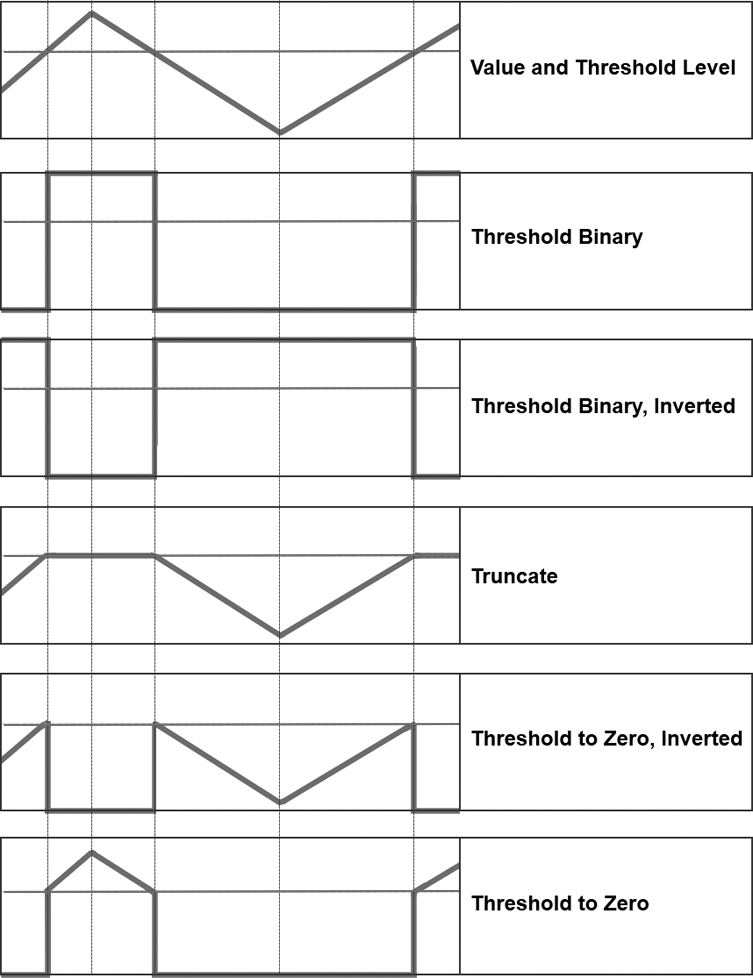
\includegraphics[width=\textwidth]{images/thresholds}
	\caption{Threshold variants in OpenCV}
	\source{\cite{learning-opencv-3}, Figure 10-4}
	\label{fig:threshold_variants}
\end{figure}

\begin{figure}
	\centering
	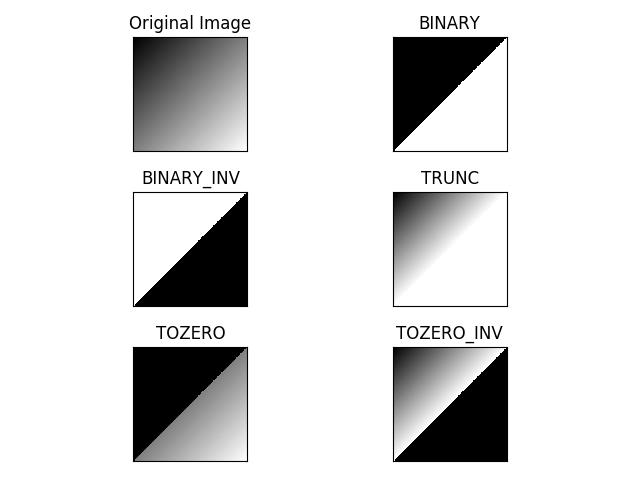
\includegraphics[width=\textwidth]{images/thresholds_example}
	\caption{Example usage of thresholds in OpenCV}
	\label{fig:threshold_examples}
\end{figure}

\section{Image Filtering}
\paragraph{Introduction}
Filtering is a technique for modifying or enhancing an image. It is used either to emphasize some features of the image or to remove some other. Images can be filtered with various low-pass filters (LPF) or high-pass filters (HPF). HPFs are useful for finding edges in the images whereas LPFs are used to remove noise and for image blurring.

\paragraph{Correlation and convolution}\cite{correlation-convolution}
This are basic operations that can be applied in order to extract information from an image. In a sense they are the simplest operations that can be performed but, nevertheless, extremely powerful and useful. Due to their simplicity they are also well understood, easy implementable and efficiently computable. Both of these operations fullfill two features:
\begin{itemize}
	\item Linearity
	\item Shift-invariance
\end{itemize}
Let us now look at correlation in 2D. Given a square filter with odd number of elements represented by a $(2N + 1)$ x $(2N + 1)$ matrix $F$ and the image matrix $I$, the results of correlation can be computed by aligning the center of the filter with a pixel. Overlapping values are then multiplied together and summed up to make the result corresponding to that given pixel. It can be written as
\begin{equation}
	(F \otimes I)(x, y) = \sum_{i = -N}^{N}\sum_{j = -N}^{N}F(i, j)I(x + i, y + j)
\end{equation}
Convolution is very similar to correlation, but the filter is flipped both horizontally and vertically beforehand. 
\begin{equation}
	(F \star I)(x, y) = \sum_{i = -N}^{N}\sum_{j = -N}^{N}F(i, j)I(x - i, y - j)
\end{equation}

\paragraph{}
Let us now see a simple example presenting difference between correlation and convolution. Equation \ref{eq:correlation} shows a very basic example of correlation.
\begin{equation}
\begin{bmatrix}
    0 & 0 & 0 & 0 & 0 & 0 & 0 \\
    0 & 0 & 0 & 0 & 0 & 0 & 0 \\
    0 & 0 & 0 & 0 & 0 & 0 & 0 \\
    0 & 0 & 0 & 1 & 0 & 0 & 0 \\
    0 & 0 & 0 & 0 & 0 & 0 & 0 \\
    0 & 0 & 0 & 0 & 0 & 0 & 0 \\
    0 & 0 & 0 & 0 & 0 & 0 & 0 \\            
\end{bmatrix}
\otimes
\begin{bmatrix}
    a & b & c \\
    d & e & f \\
    g & h & i
\end{bmatrix}
=
\begin{bmatrix}
    0 & 0 & 0 & 0 & 0 & 0 & 0 \\
    0 & 0 & 0 & 0 & 0 & 0 & 0 \\
    0 & 0 & i & h & g & 0 & 0 \\
    0 & 0 & f & e & d & 0 & 0 \\
    0 & 0 & c & b & a & 0 & 0 \\
    0 & 0 & 0 & 0 & 0 & 0 & 0 \\
    0 & 0 & 0 & 0 & 0 & 0 & 0 \\            
\end{bmatrix}
\label{eq:correlation}
\end{equation}

\paragraph{}
Equation \ref{eq:convolution}, on the other hand, presents a convolution. We can see that it is indeed equivalent to a correlation with a flipped filter.

\begin{equation}
\begin{array}{l}
\begin{bmatrix}
    0 & 0 & 0 & 0 & 0 & 0 & 0 \\
    0 & 0 & 0 & 0 & 0 & 0 & 0 \\
    0 & 0 & 0 & 0 & 0 & 0 & 0 \\
    0 & 0 & 0 & 1 & 0 & 0 & 0 \\
    0 & 0 & 0 & 0 & 0 & 0 & 0 \\
    0 & 0 & 0 & 0 & 0 & 0 & 0 \\
    0 & 0 & 0 & 0 & 0 & 0 & 0 \\            
\end{bmatrix}
\star
\begin{bmatrix}
    a & b & c \\
    d & e & f \\
    g & h & i
\end{bmatrix}
= \\ \\
=
\begin{bmatrix}
    0 & 0 & 0 & 0 & 0 & 0 & 0 \\
    0 & 0 & 0 & 0 & 0 & 0 & 0 \\
    0 & 0 & 0 & 0 & 0 & 0 & 0 \\
    0 & 0 & 0 & 1 & 0 & 0 & 0 \\
    0 & 0 & 0 & 0 & 0 & 0 & 0 \\
    0 & 0 & 0 & 0 & 0 & 0 & 0 \\
    0 & 0 & 0 & 0 & 0 & 0 & 0 \\            
\end{bmatrix}
\otimes
\begin{bmatrix}
    i & h & g \\
    f & e & d \\
    c & b & a
\end{bmatrix}
=
\begin{bmatrix}
    0 & 0 & 0 & 0 & 0 & 0 & 0 \\
    0 & 0 & 0 & 0 & 0 & 0 & 0 \\
    0 & 0 & a & b & c & 0 & 0 \\
    0 & 0 & d & e & f & 0 & 0 \\
    0 & 0 & g & h & i & 0 & 0 \\
    0 & 0 & 0 & 0 & 0 & 0 & 0 \\
    0 & 0 & 0 & 0 & 0 & 0 & 0 \\            
\end{bmatrix}
\end{array}
\label{eq:convolution}
\end{equation}

\paragraph{}
The key distinction before the two operations is the associative property of convolution:
\begin{equation}
	\forall F, G - filters \quad \forall I - image: F \star (G \star I) = (F \star G) \star I
\end{equation}
This property is useful when there is need to convolve image with multiple filters. It is computationally faster to precompute the final filter as convolution of original filters and apply just one convolution to the input image. Convolutions are used for image processing operations such as smoothing whereas correlations are useful for matching templates.
One final notice, that for symmetrical filters convolution and correlation are identical.

\paragraph{Image blurring}
To achieve smoothing effect, the image is convolved with a LPF kernel. This particular type of filtering removes high frequency content from the image (for example noise). Unfortunately, edges also can be blurred a bit while applying this operation, although there are also smoothing filters that prevent edges from being blurred. The OpenCV library provides user with various filters amongst which the most popular ones are:
\begin{itemize}
	\item Averaging - it takes the average of all the pixels under kernel area
	\item Gaussian - instead of box filter, a Gaussian kernel is used
	\item Median - in this case the median value of all the pixels under kernel area is used
	\item Bilateral - slower compared to other filters, but it keeps edges sharp
\end{itemize}

\section{Morphological Transformations}
\paragraph{}
Morphological transformations are operations based on the image shape. Two inputs are needed to perform such a transformation, one being the original image whereas the other, called kernel, decides the nature of operation. It is performed on binary images, with black background (having value 0) and white foreground (having value 1). Two most basic ones are erosion and dilation which will now be presented.

\paragraph{}
\textbf{Erosion} - erodes away the boundaries of the foreground object. It is performed by sliding the kernel over the image. For each pixel the following equation is applied.

\begin{equation}
	Erosion(pixel, kernel) = \begin{cases}
		1 & \text{if all the pixels under $kernel$ are 1}\\
		0 & \text{otherwise}
	\end{cases}
\end{equation}

When the output of erosion is 0, the pixel is said to be eroded.

\paragraph{}
\textbf{Dilation} - on the other hand, it is the opposite of erosion. 

\begin{equation}
	Erosion(pixel, kernel) = \begin{cases}
		1 & \text{if at least one pixel under $kernel$ is 1}\\
		0 & \text{otherwise}
	\end{cases}
\end{equation}

\paragraph{}
Figure \ref{fig:morphological_examples} shows both erosion and dilation applied to some simple image. It also presents one more morphological transformation, which is just a combination of both of them, \textbf{gradient} - a difference between dilation and erosion of an image.

\begin{figure}[H]
	\centering
	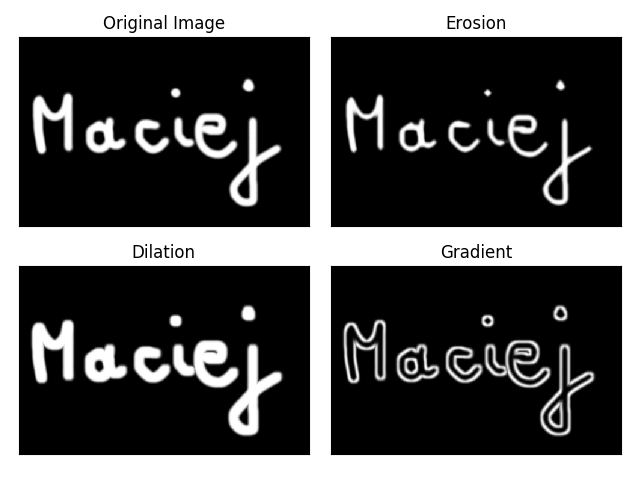
\includegraphics[width=\textwidth]{images/morphological}
	\caption{Example of morphological transformations}
	\label{fig:morphological_examples}
\end{figure}

\section{Finding Contours}
\paragraph{}
A contour is a list of points that represent, in one way or another, a curve in an image.\cite{learning-opencv-3} They come in handy for analysing the shape of an object, for its detection and for recognition. For better results it is good to use binary images, so the process of contours finding should be applied after thresholding or edge detecting.

\paragraph{}
Figure \ref{fig:preprocessing} shows what the process of finding contours can lead to - detecting the shape of an object.

\section{Edge Detection}
\subsection{Derivatives and edges}
An edge is a place of a sudden discontinuity in an image, which can arise from surface normal, surface color, depth, illumination, or other discontinuities. This rapid change in the image intensity function can be observed in places where the first derivative of this function has local extrema (see Figure \ref{fig:edge-detection}).\cite{edge-detection}
\begin{figure}[H]
     \centering
     \subfloat[Original Image]{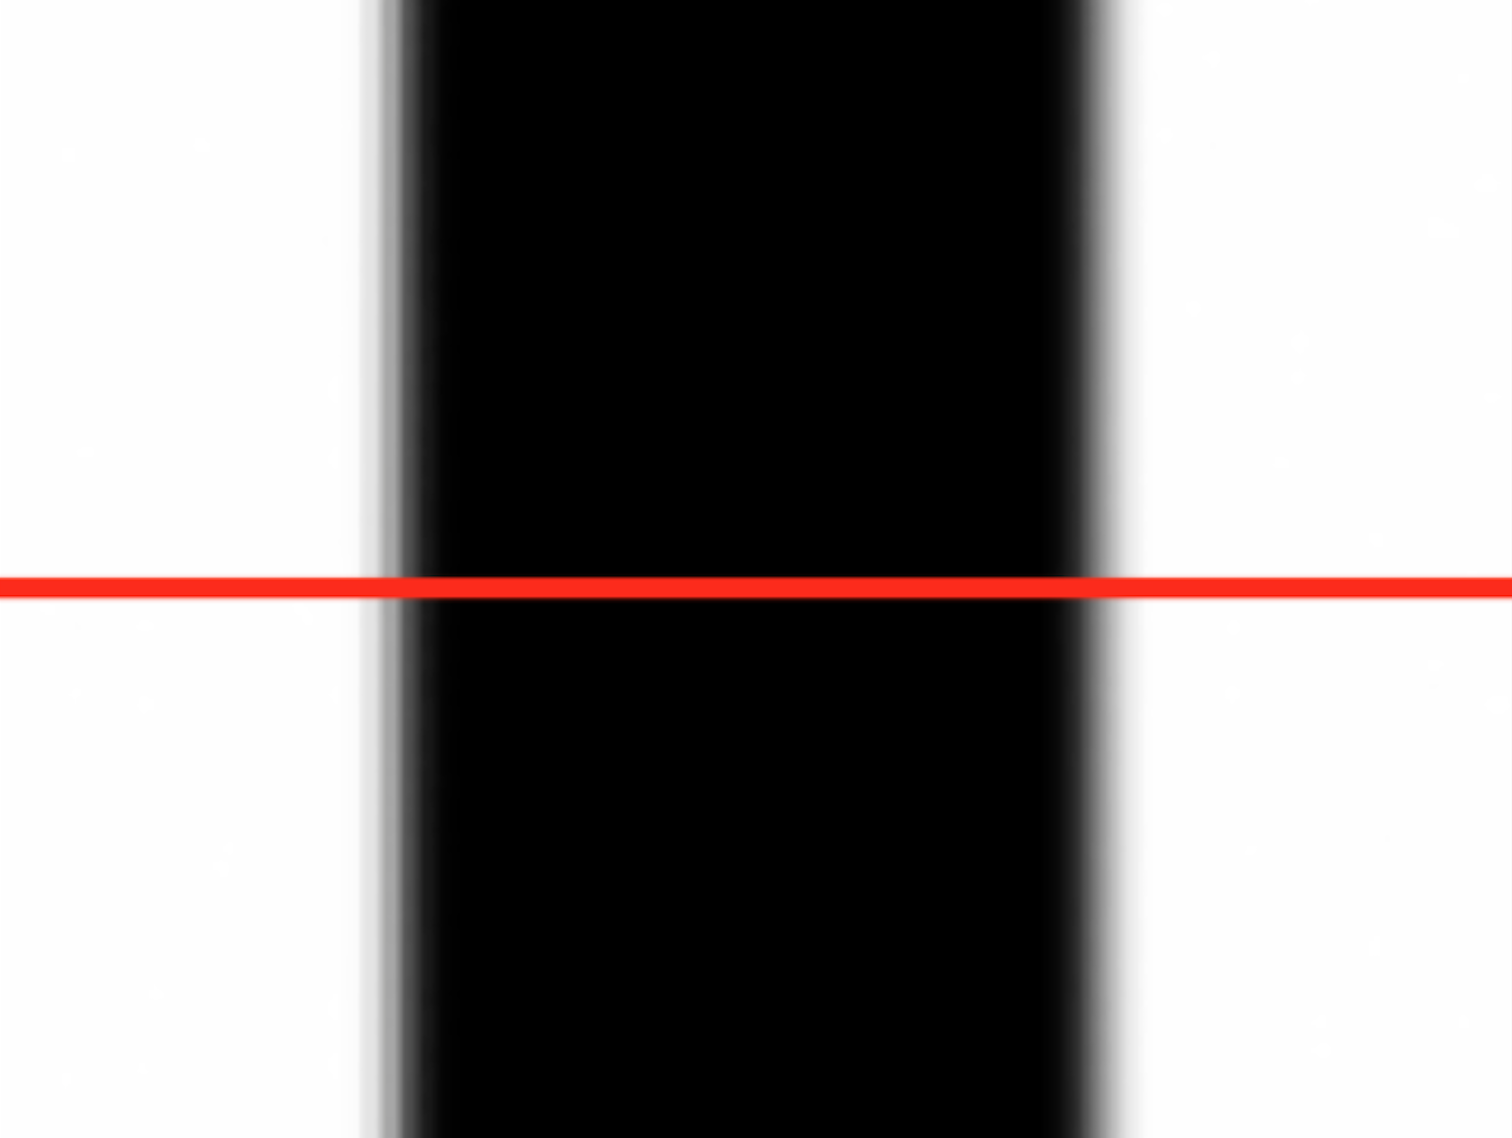
\includegraphics[width=0.5\textwidth]{images/edge_image}}
     \vfill
     \subfloat[Intensity along the specified line]{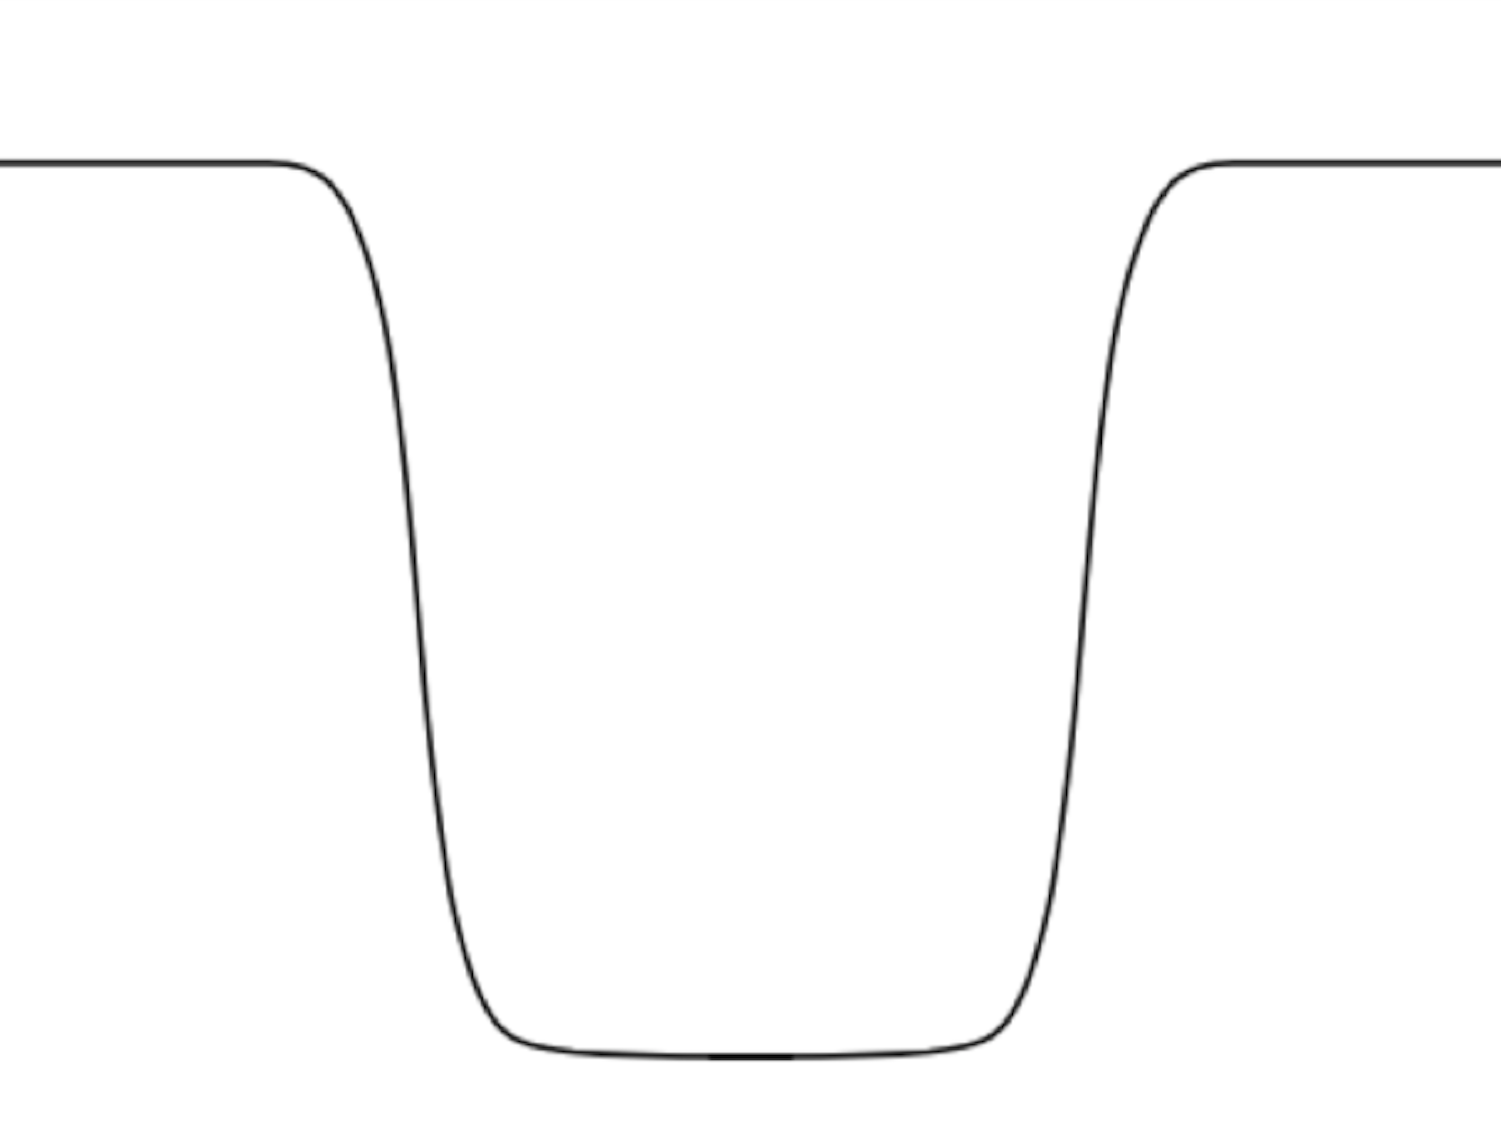
\includegraphics[width=0.5\textwidth]{images/edge_intensity_function}}
     \vfill
     \subfloat[Derivative of the intensity function]{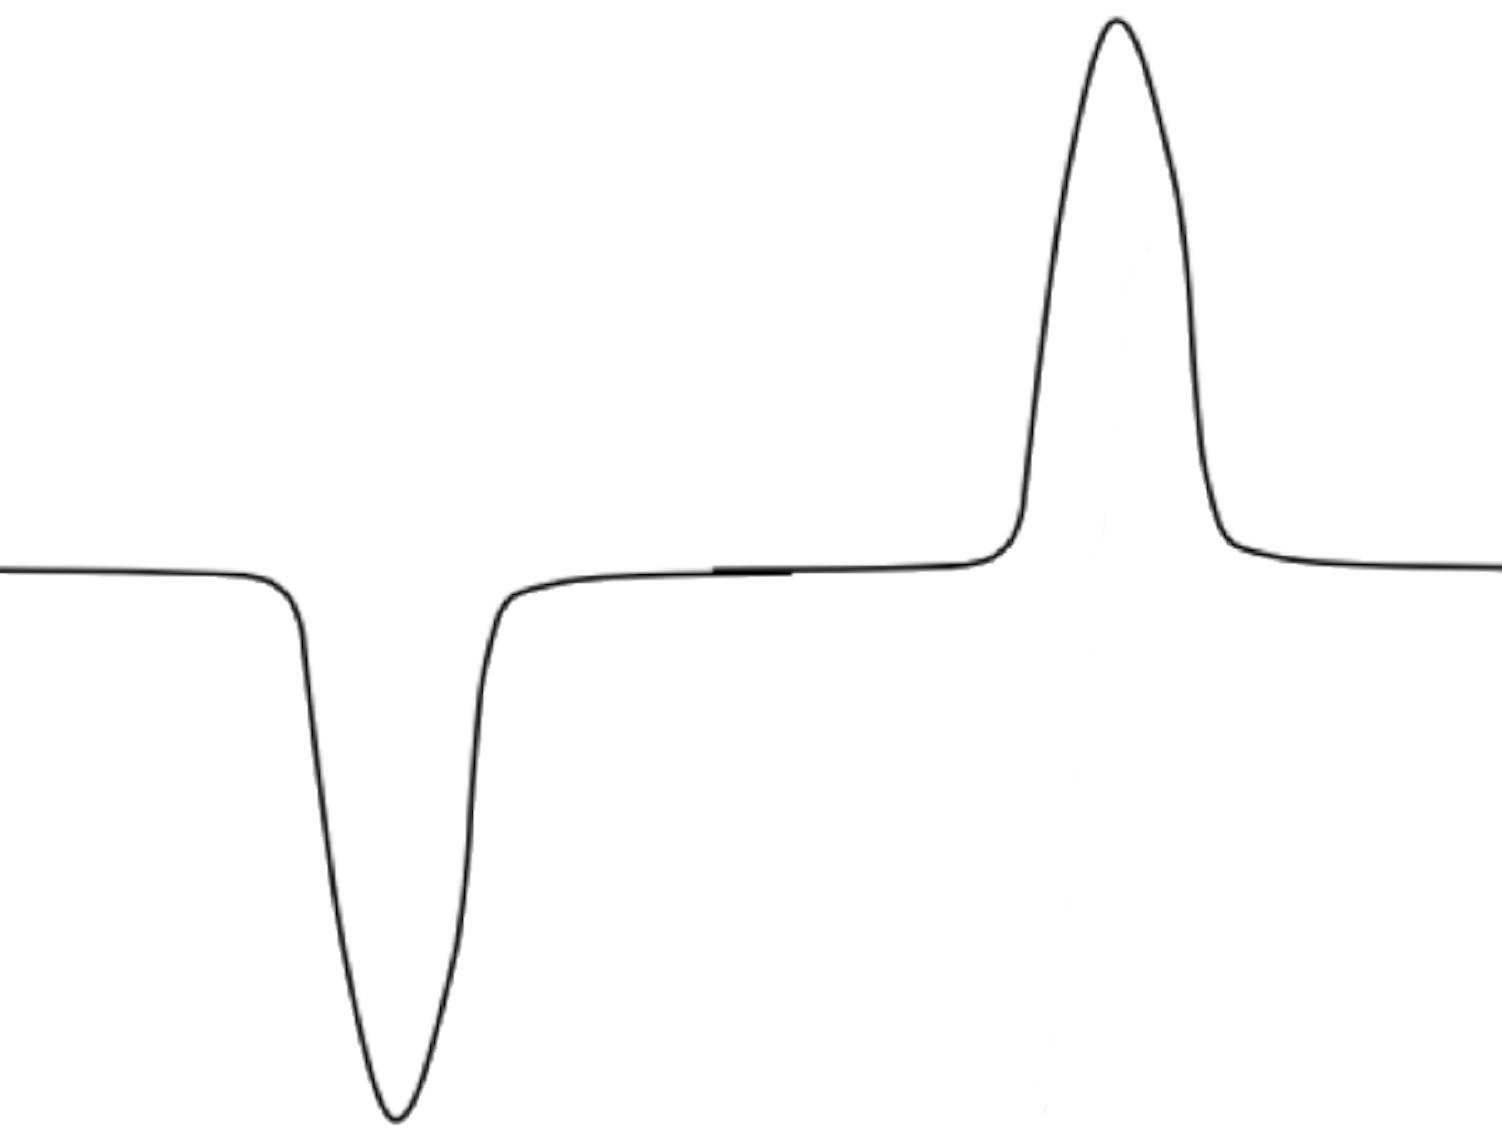
\includegraphics[width=0.5\textwidth]{images/edge_first_derivative}}
     \caption{Edge detection}
     \label{fig:edge-detection}
     \source{\cite{lazebnik-edge}, Slide 4}
\end{figure}

\subsection{Image gradient}
The gradient of a scalar function $f(x, y)$, where $f: \mathbb{R}^2 \rightarrow \mathbb{R}$ is denoted $\nabla f$ (where $\nabla$ is the nabla symbol). In two-dimensional Cartesian coordinate system with the Euclidean metric, the gradient, if exists, is given by:
\begin{equation}
	\nabla f = [\frac{\partial f}{\partial x}, \frac{\partial f}{\partial y}]
\end{equation}
It points in the direction of most rapid increase in intensity and that direction is given by:
\begin{equation}
	\theta = tan^{-1}(\frac{\frac{\partial f}{\partial y}}{\frac{\partial f}{\partial x}})
\end{equation}
And, finally, the \textit{amount of change} is given by the gradient magnitude:
\begin{equation}
	\parallel \nabla f \parallel = \sqrt{(\frac{\partial f}{\partial x})^2 + (\frac{\partial f}{\partial y})^2}
\end{equation}
Remember, that for 2D function partial derivative is defined as:
\begin{equation}
	\frac{\partial f(x,y)}{\partial x} = \lim_{\epsilon \to 0} \frac{f(x + \epsilon, y) - f(x, y)}{\epsilon}
\end{equation}
But for discrete data this definition needs to be approximated using finite differences:
\begin{equation}
	\frac{\partial f(x,y)}{\partial x} \approx \frac{f(x + 1, y) - f(x, y)}{1} \approx f(x + 1, y) - f(x, y)
\end{equation}
In order to obtain an operator (a kernel) that implements the definition of the discrete gradient, we end up with averaging "left" and "right" derivative and obtain the kernel:
\[
\frac{1}{2}
(\begin{bmatrix}
    0 & 0 & 0 \\
    -1 & 1 & 0 \\
    0 & 0 & 0
\end{bmatrix}
+
\begin{bmatrix}
    0 & 0 & 0 \\
    0 & -1 & 1 \\
    0 & 0 & 0
\end{bmatrix})
=
\begin{bmatrix}
    0 & 0 & 0 \\
    \frac{-1}{2} & 0 & \frac{1}{2} \\
    0 & 0 & 0
\end{bmatrix}
\]

{\renewcommand{\arraystretch}{2}
\begin{table}[H]
	\centering
	\begin{tabular}{ccc}
		 & \textbf{X} & \textbf{Y} \\
		\hline
		\\
		\textbf{Sobel} & $\begin{bmatrix} -1 & 0 & 1 \\ -2 & 0 & 2 \\ -1 & 0 & 1 \end{bmatrix}$ & $\begin{bmatrix} 1 & 2 & 1 \\ 0 & 0 & 0 \\ -1 & -2 & -1\end{bmatrix}$ \\
		\\
		\hline
		\\
		\textbf{Prewitt} & $\begin{bmatrix} -1 & 0 & 1 \\ -1 & 0 & 1 \\ -1 & 0 & 1 \end{bmatrix}$ & $\begin{bmatrix} 1 & 1 & 1 \\ 0 & 0 & 0 \\ -1 & -1 & -1 \end{bmatrix}$ \\
		\\
		\hline
		\\
		\textbf{Roberts} & $\begin{bmatrix} 1 & 0 \\ 0 & -1 \end{bmatrix}$ & $\begin{bmatrix} 0 & 1 \\ -1 & 0 \end{bmatrix}$ \\
		\\
		\hline
	\end{tabular}
	\caption{Some of the well-known gradient kernels}
\end{table}
}
In the real world the intensity function is affected by noise and may look like in Figure \ref{fig:noise_intensity_function}
\begin{figure}[H]
	\centering
	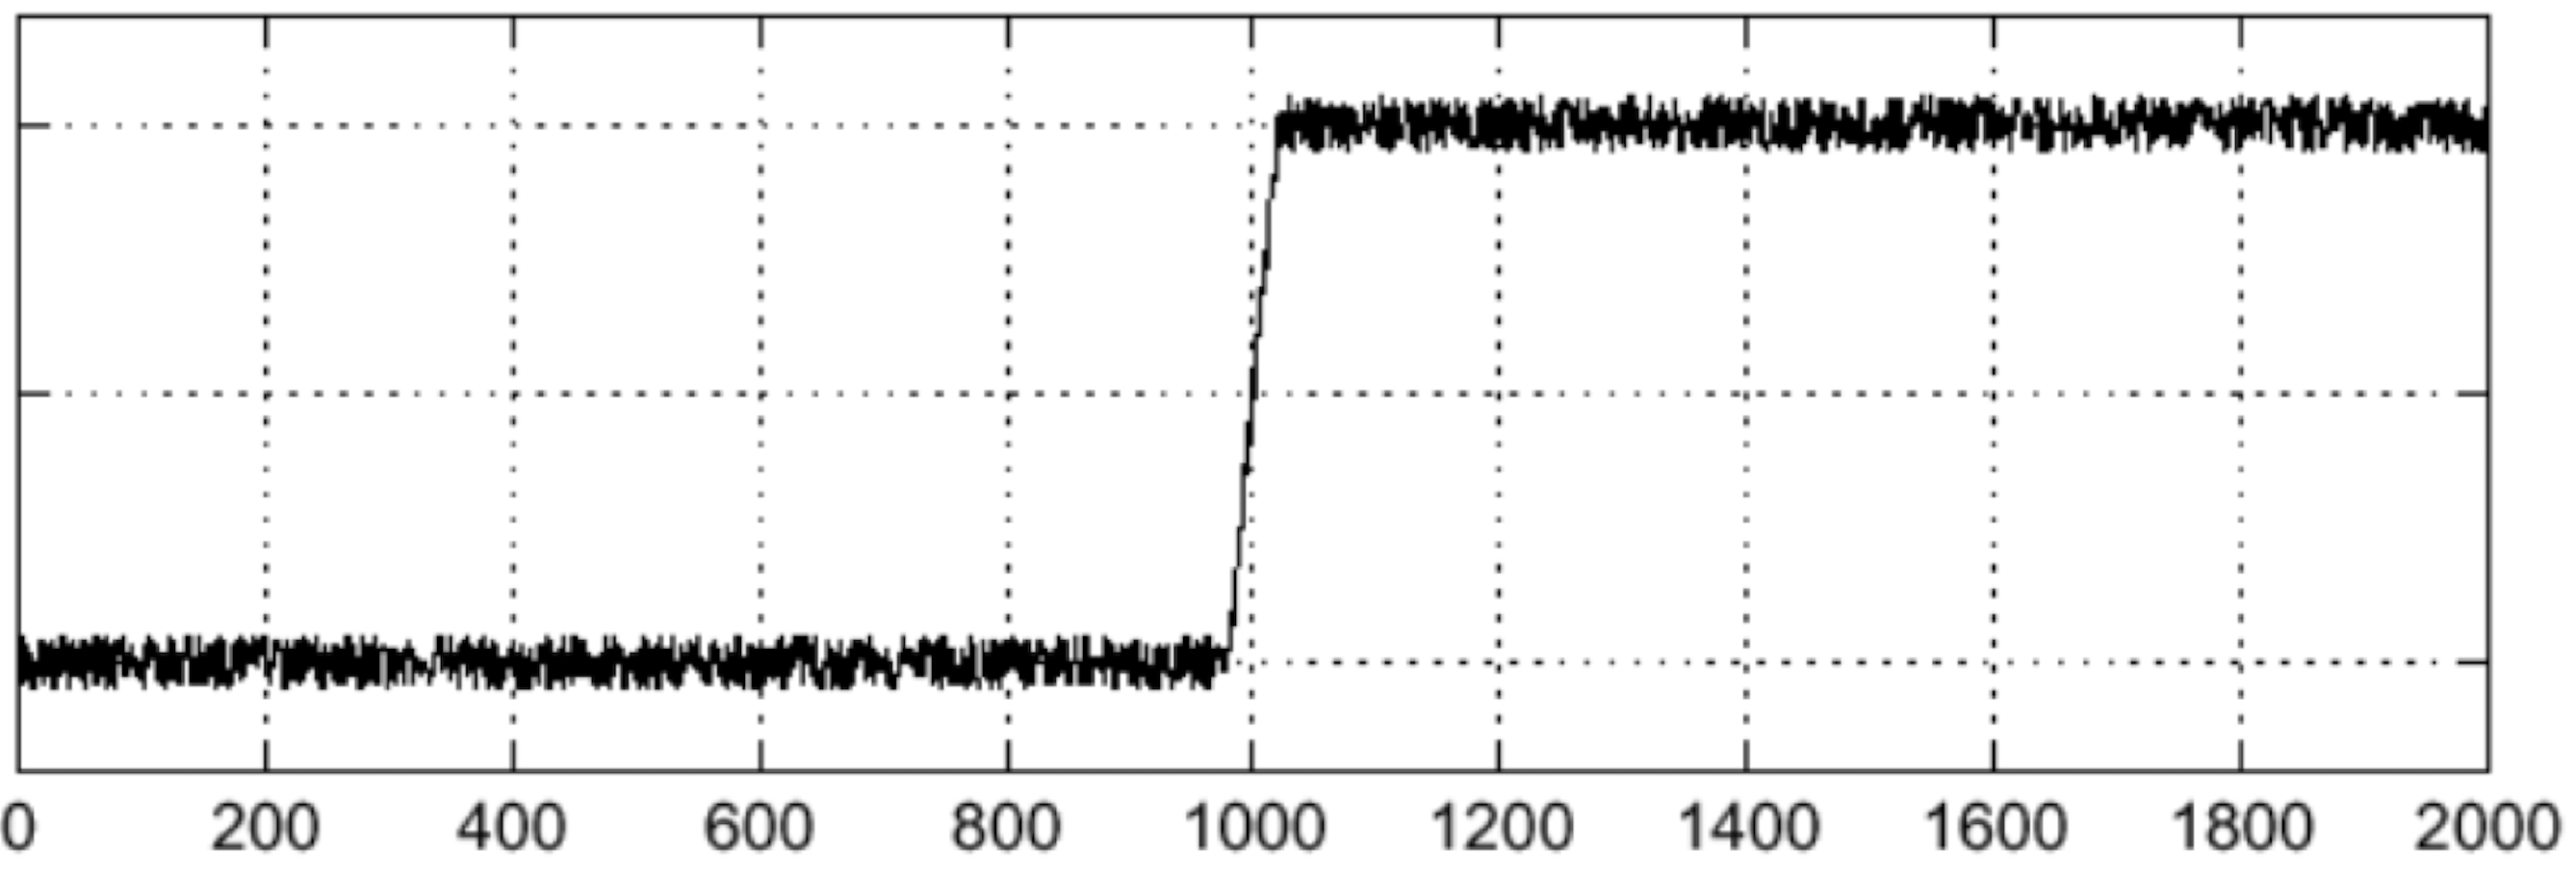
\includegraphics[width=\textwidth]{images/noise_intensity_function}
	\caption{Intensity function affected by noise}
	\source{\cite{lazebnik-edge}, Slide 10}
	\label{fig:noise_intensity_function}
\end{figure}
This can cause the result of applying the derivative operator to be unable to tell where the edge might be (see Figure \ref{fig:noise_derivative})
\begin{figure}[H]
	\centering
	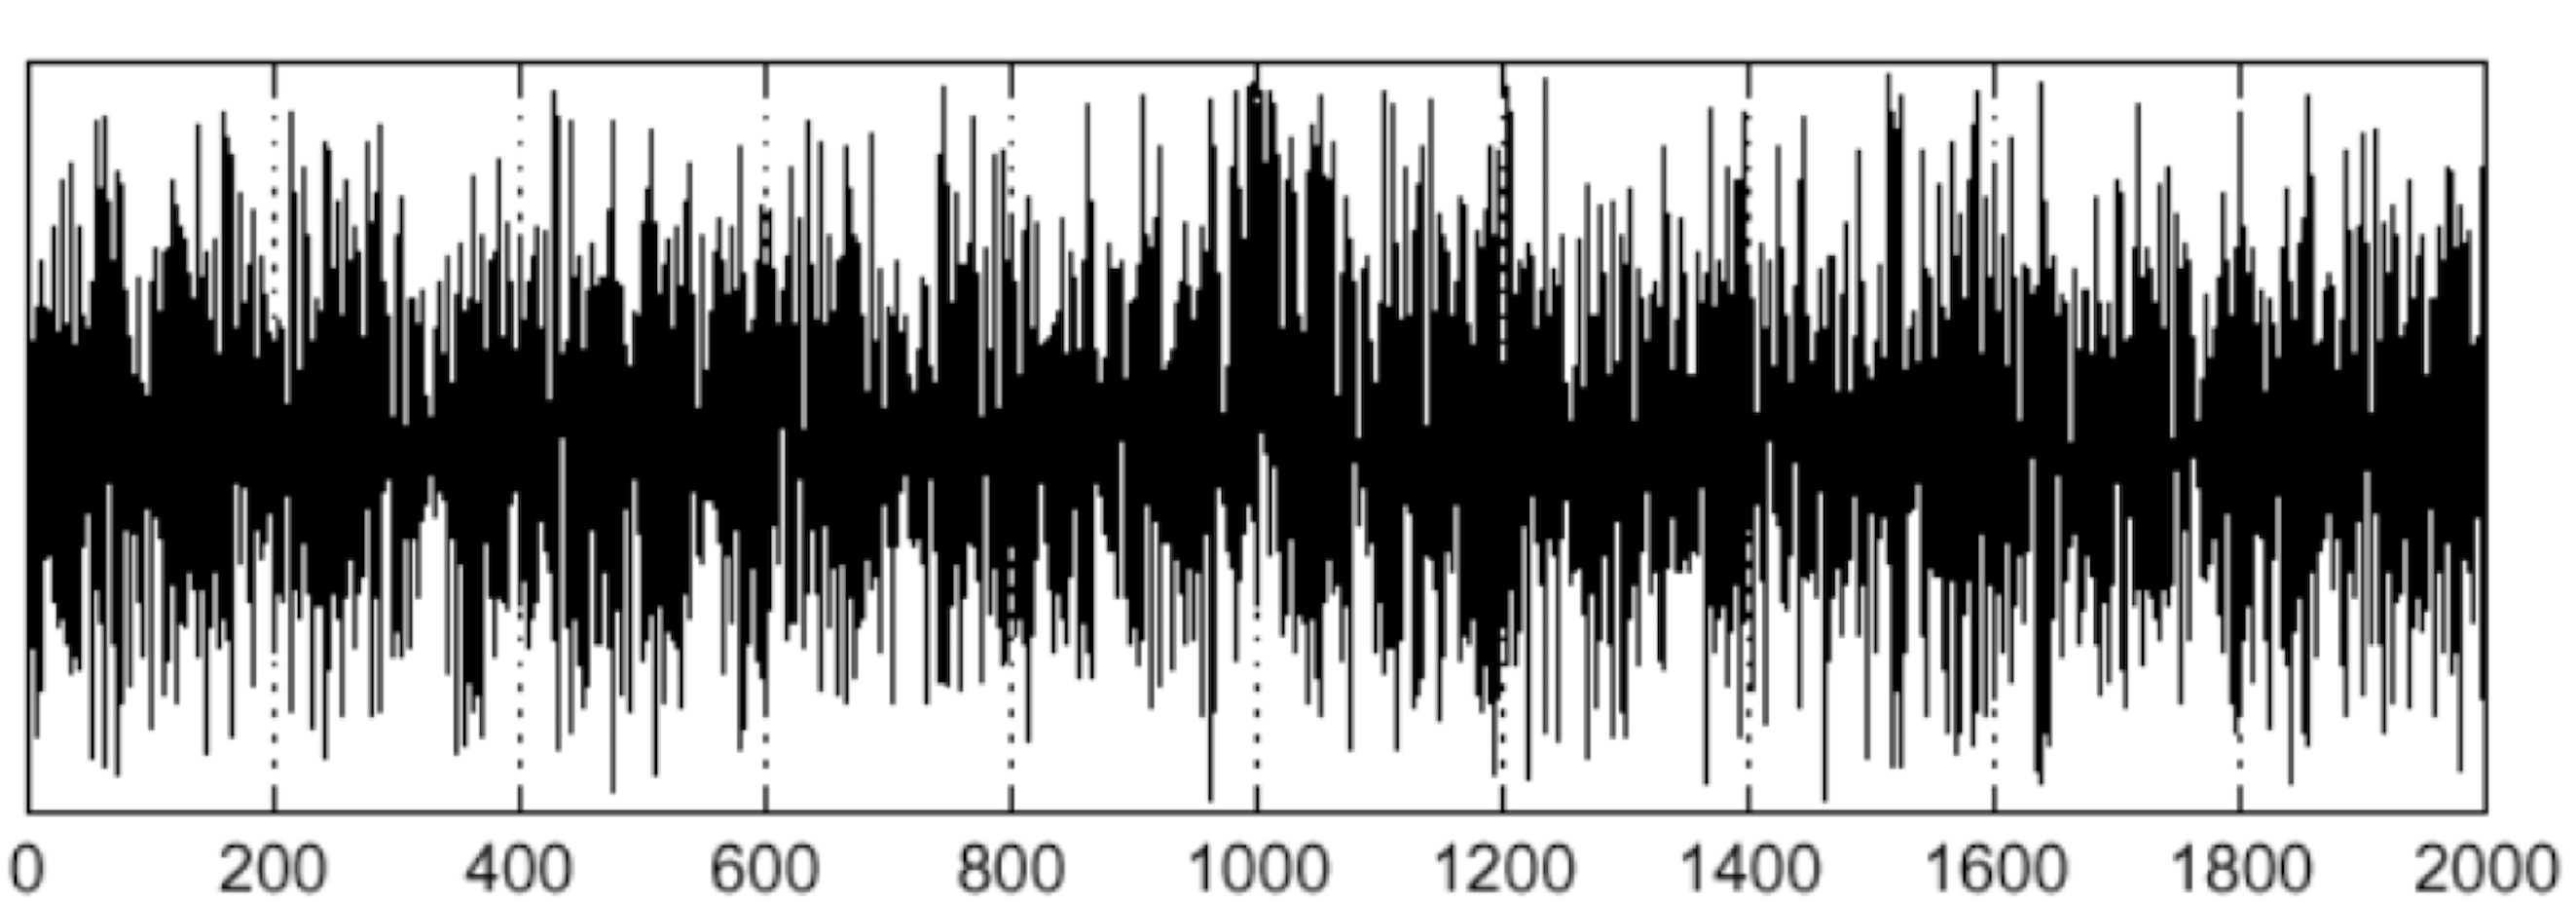
\includegraphics[width=\textwidth]{images/noise_derivative}
	\caption{Derivative of the intensity function affected by noise}
	\source{\cite{lazebnik-edge}, Slide 10}
	\label{fig:noise_derivative}
\end{figure}
\begin{figure}[H]
	\centering
	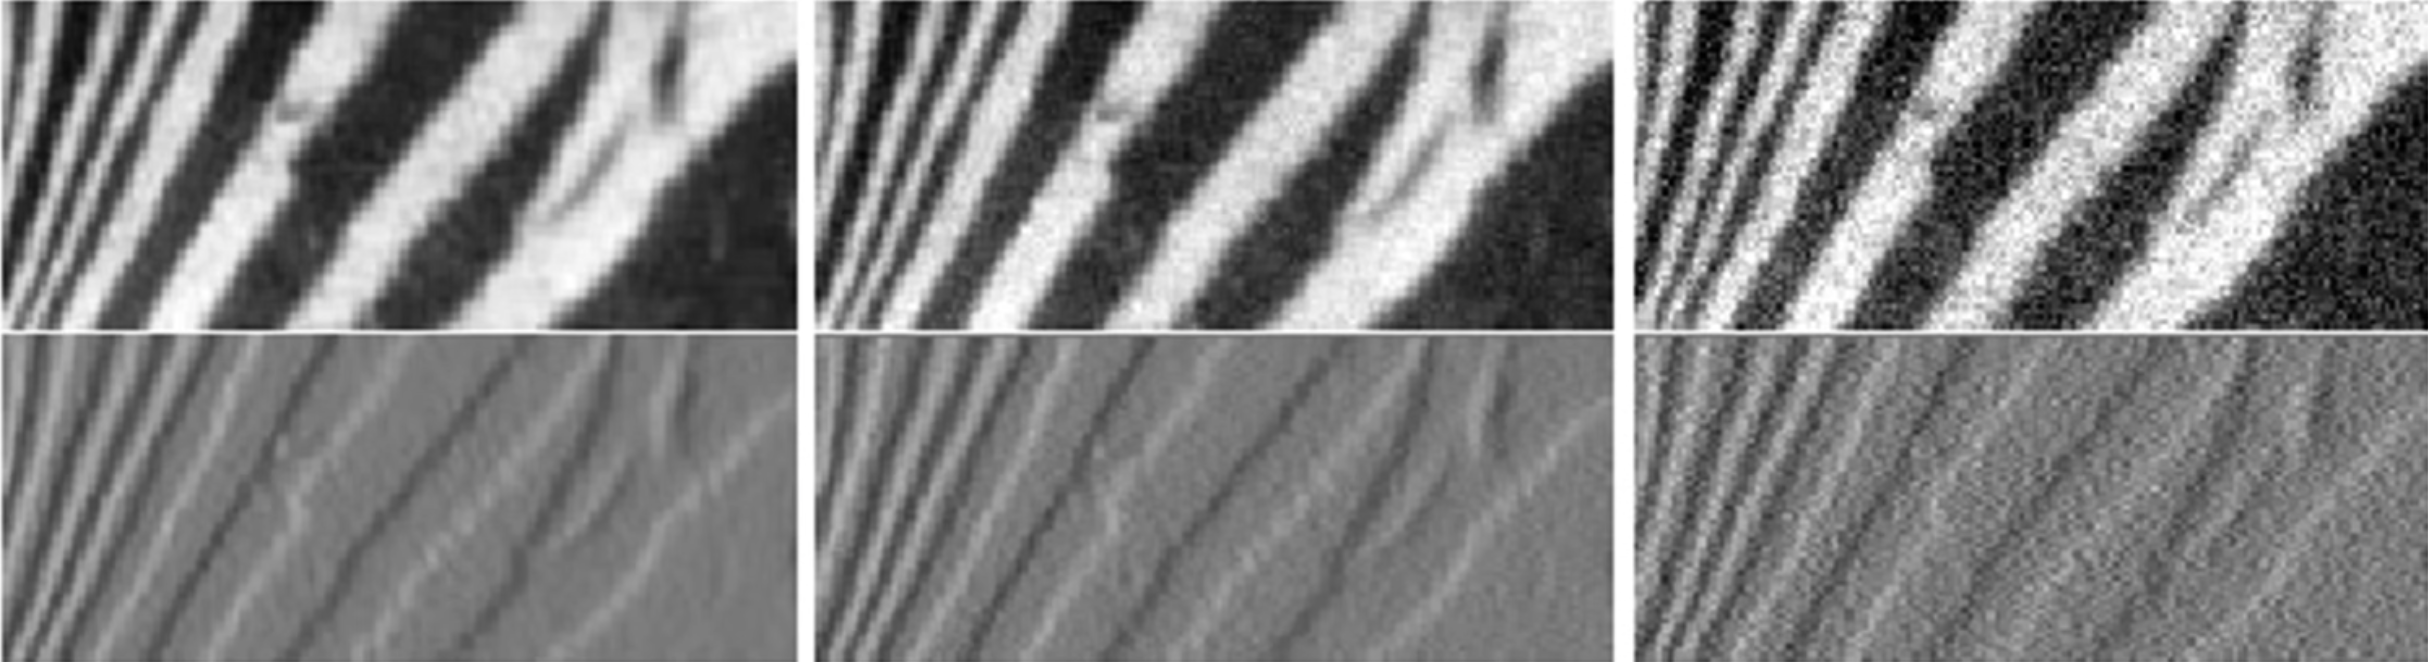
\includegraphics[width=\textwidth]{images/noise_impact}
	\caption{Noise impact on the gradient image}
	\source{\cite{modern-approach}, Figure 8.10}
	\label{fig:noise_impact}
\end{figure}

\subsection{Edge detection in general\cite{digital-image-processing}}
Primary edge detection steps include:
\begin{itemize}
	\item Smoothing derivatives to suppress noise and compute gradient
	\item Threshold to find regions of "significant" gradient
	\item Thinning to get localized edge pixels
	\item Connecting edge pixels
\end{itemize}

\subsection{Canny Edge Detection}
In particular, Canny edge operator consists of following steps\cite{canny-edge}:
\begin{enumerate}
	\item Filtering the image with derivative of Gaussian
	\item Finding the magnitude and the orientation of the gradient
	\item Performing non-maximum suppression: thinning multi-pixel wide ridges (as the edges may have been broadened in step 1.) down to single pixel width
	\item Linking and thresholding (hysteresis). To perform this step two thresholds are defined: low and high. Then it continues as follows:
	\begin{enumerate}
		\item The high threshold is applied to detect strong edge pixels
		\item Strong edge pixels are linked to form strong edges
		\item The low threshold is applied to find weak, but plausible, edge pixels
		\item Strong edges are extended to follow weak edge pixels
	\end{enumerate}
\end{enumerate}

\section{Hough Lines Detection}\label{sec:hough_lines}
\paragraph{Voting}
is a general technique where we let all the features vote for all models that are compatible with it.
\begin{enumerate}
	\item Cycle through features, each casting votes for model parameters.
	\item Look for model parameters that receive a lot of votes.
\end{enumerate}

\paragraph{Hough Line Transform}
is a voting technique that can be used to answer all of the following questions\cite{introduction-to-computer-vision}:
\begin{itemize}
	\item Given points that belong to a line, what is the line?
	\item How many lines are there?
	\item Which points belong to which lines?
\end{itemize}
In order to use Hough Line Transform, the image should be binary. The most common approach is to convert color image to grayscale, then apply edge detection to obtain the edge pixels. This binary image then undergoes Hough transformation that outputs a set of lines that were found. The main idea of this algorithm is as follows:
\begin{enumerate}
	\item Each edge pixel votes for compatible lines
	\item Look for lines that got many votes
\end{enumerate}

\paragraph{Line representations}
Let us now look at the possible representations of a line. The simplest and most widely used one is using Cartesian coordinates (see Figure \ref{fig:line_cartesian}):
\begin{equation}
	y = m x + b
\end{equation}
where $m$ represents the slope and $b$ the intercept with Y-axis.
\begin{figure}[H]
	\centering
	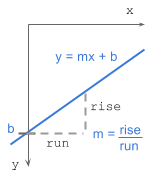
\includegraphics[width=0.3\textwidth]{images/hough_cartesian_equation}
	\caption{Line represented in Cartesian coordinates}
	\source{\cite{hough-lines-python}}
	\label{fig:line_cartesian}
\end{figure}
Other possible representation of a line is in polar coordinates (see Figure \ref{fig:line_polar}):
\begin{equation}
	\rho = x \cos\theta + y \sin\theta
\end{equation}
where non-negative $\rho$ represents the perpendicular distance from origin to the line and $\theta \in [0, 2\pi)$ the angle the perpendicular makes with with the X-axis.
\begin{note}
	The OpenCV implementation of the Hough Lines algorithm returns the $\theta$ with values from range $[0, \pi]$ and allows negative $\rho$.
\end{note}
\begin{figure}[H]
	\centering
	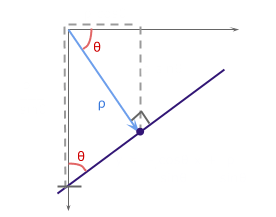
\includegraphics[width=0.3\textwidth]{images/hough_polar}
	\caption{Line represented in polar coordinates}
	\source{\cite{hough-lines-python}}
	\label{fig:line_polar}
\end{figure}

\paragraph{Hough space}
Let us now consider Image Space to be represented in polar coordinates. A line is then represented by some $\rho$ and $\theta$. We can draw such a point in $(\rho, \theta)$ coordinates that will be called \textbf{Hough space}.\cite{hough-lines}
\begin{figure}[H]
	\centering
	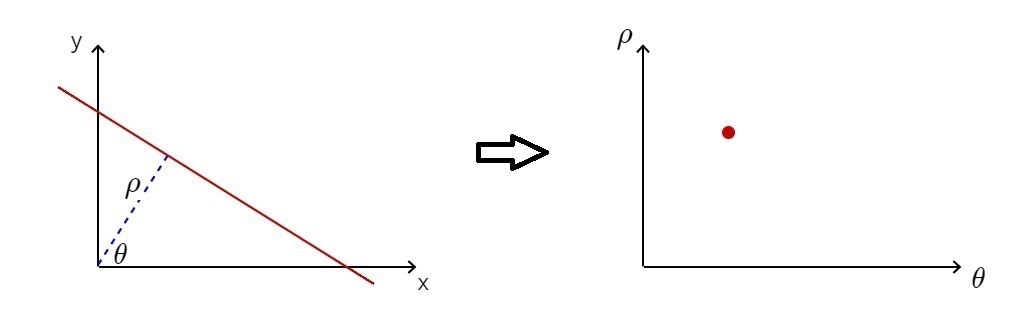
\includegraphics[width=\textwidth]{images/line_to_hough_space}
	\caption{Line represented in Hough space}
	\source{\cite{hough-lines}}
	\label{fig:line_hough_space}
\end{figure}
\begin{figure}[H]
	\centering
	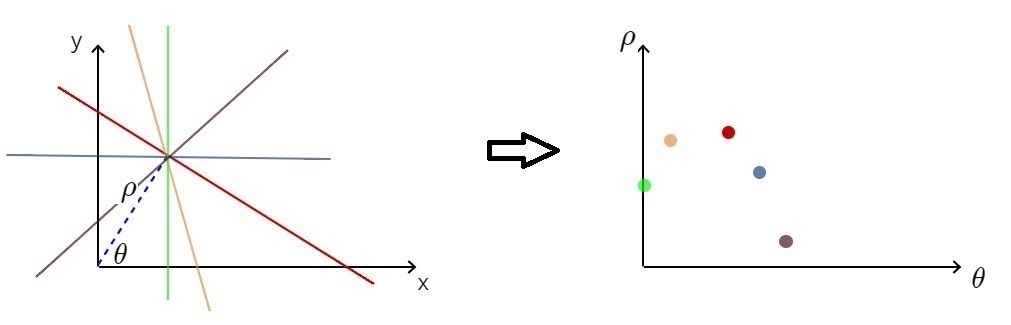
\includegraphics[width=\textwidth]{images/lines_to_hough_space}
	\caption{Bunch of lines with common point represented in Hough space}
	\source{\cite{hough-lines}}
	\label{fig:bunch_of_lines_hough_space}
\end{figure}
It turns out that a point in image space results in a sinusoid in Hough space.
\begin{figure}[H]
	\centering
	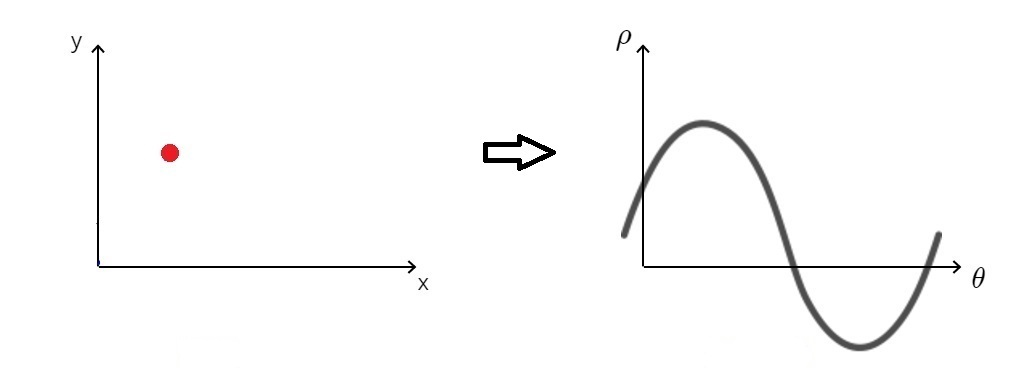
\includegraphics[width=\textwidth]{images/point_to_sinusoid}
	\caption{Point in image space represented as sinusoid in Hough space}
	\source{\cite{hough-lines}}
	\label{fig:point_to_sinusoid}
\end{figure}
\begin{table}[H]
	\centering
	\begin{spacing}{1.5}
	\begin{tabular}{|l|l|}
		\hline
		\textbf{Image space} & \textbf{Hough space} \\ [0.5ex]
		\hline
		Straight line & Point \\ [0.5ex]
		\hline
		Point & Sinusoid \\ [0.5ex]
		\hline
	\end{tabular}
	\end{spacing}
	\caption{Duality between image space and Hough space}
\end{table}
Finally, take a look at points that are forming a line in image space and their corresponding sinusoids in Hough space (Figure \ref{fig:line_detection_in_hough_space}). We can see, that all of the sinusoids intersect at exactly one point that represents the $(\rho, \theta)$ parameters of our line in image space.
\begin{figure}[H]
	\centering
	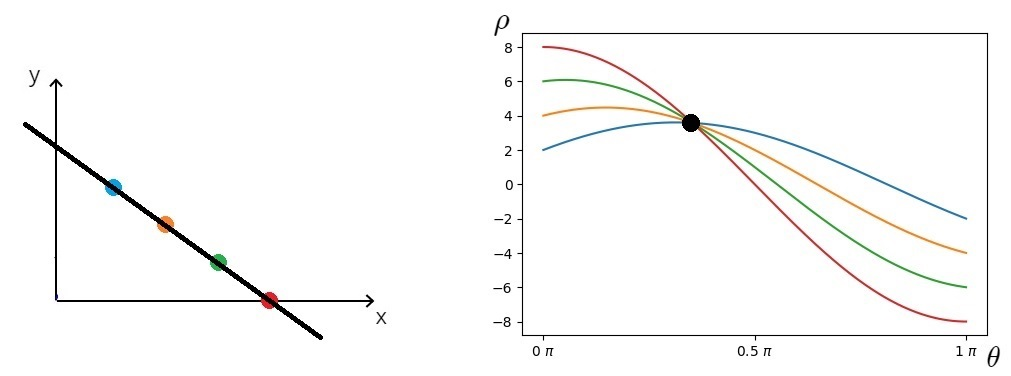
\includegraphics[width=\textwidth]{images/points_to_sinusoids}
	\caption{Detecting a line in Hough space}
	\source{\cite{hough-lines}}
	\label{fig:line_detection_in_hough_space}
\end{figure}

\paragraph{Hough Line Transform}
Let us now look how it all works for actually finding the lines. As mentioned earlier, the algorithm uses a voting technique, so we let each edge pixel to cast its votes. An accumulator (a matrix) is created to hold those votes. Looping over the edge pixels, we generate sinusoidal curves that correspond to this point in Hough space for each $\theta$ in range $[0, \pi]$ given some step ($\delta$). For that value of $\theta$ the corresponding $\rho$ is computed (from the line equation: $\rho = x\cos\theta + y\sin\theta$). Such a $(\theta, \rho)$ pair increments corresponding count of votes in the accumulator matrix. Then next value of $\theta$ is taken and the procedure repeats. This continues up until $\theta$ is equal to $\pi$  and for each of those values votes are "casted". Then next edge pixel is taken and is voting. The procedure ends when no edge pixel is left to vote. Cells from the accumulator matrix that have a lot of votes correspond to lines in image space.

\begin{algorithm}
	\begin{spacing}{1.5}
	\begin{algorithmic}[1]
		\Function{hough\_line\_transform}{$edge\_image$}
			\State Initialize $H[\rho, \theta] = 0$
			\For{$edge\_pixel$ \textbf{in} $edge\_image$}
				\For{$\theta$ \textbf{in} \textbf{range}$(0, 180, \delta)$}
					\State $\rho \gets x\cos\theta + y\sin\theta$
					\State $H[\rho, \theta] += 1$
				\EndFor
			\EndFor
			\State Find value(s) of $(\rho, \theta)$ where $H[\rho, \theta]$ is a local maximum
		\EndFunction
	\end{algorithmic}
	\end{spacing}
	\caption{Hough Line Transform}
\end{algorithm}

\begin{note}
It is worth noting, that the accuracy of this algorithm highly depends on the number of cells in the accumulator matrix. If, for example the step $\delta$ was $45^{\circ}$ we would only have $\{0^{\circ}, 45^{\circ}, 90^{\circ}, 135^{\circ}, 180^{\circ}\}$ as the cells for $\theta$ value. The voting process would then be highly inaccurate. It also cannot be to granular, because this technique depends on relatively high number of votes to be casted in a small region.
\end{note}

Figure \ref{fig:hough-line-transform} shows an edge image that contains two visible lines $(a)$. Applying the Hough Line Transform outputs the results that are visualized on image $(b)$. Sinusoidal curves that correspond to edge pixels are shown. We can observe two very bright spots where a large number of curves intersect. This means that those spots (some $(\rho, \theta)$ pairs) have gained a lot of votes in the accumulator matrix. Hence, they are yield as lines that are marked on the output image $(c)$.

\begin{figure}[H]
     \centering
     \subfloat[Input image]{
\includegraphics[width=0.3\textwidth]{images/hough_input}}
     \hfill
     \subfloat[Hough Line Transform]{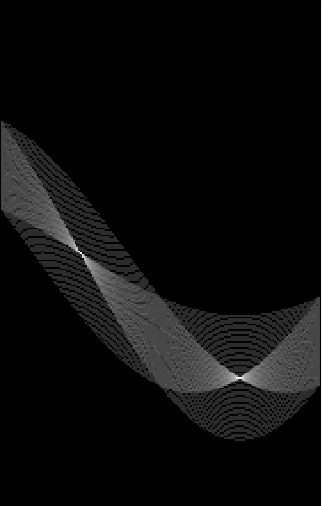
\includegraphics[width=0.3\textwidth]{images/hough_transform}}
     \hfill
     \subfloat[Lines found]{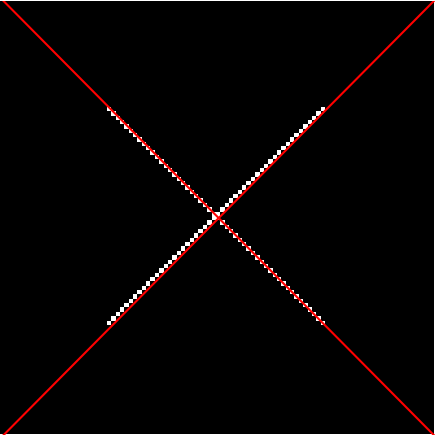
\includegraphics[width=0.3\textwidth]{images/hough_output}}
     \caption{Example of applying Hough Line Transform}
     \source{\url{http://scikit-image.org/docs/0.9.x/auto_examples/plot_line_hough_transform.html}}
     \label{fig:hough-line-transform}
\end{figure}


\chapter{Development Environment}
\lstdefinestyle{mystyle}{
    breakatwhitespace=false,         
    breaklines=true,                 
    captionpos=b,                    
    keepspaces=true,                 
    numbers=left,                    
    numbersep=15pt,                  
    showspaces=false,                
    showstringspaces=false,
    showtabs=false,                  
    tabsize=2
}
 
\lstset{style=mystyle}

\section{OpenCV}
\paragraph{}
OpenCV (\url{https://opencv.org/}) is an open source computer vision library available under BSD licence. Its' alpha version was released in 1999 by an Intel Corporations' employee with hopes of a quicker and broader evolution of computer vision and artificial intelligence development. The library is primarily written in C and C++ and runs under any modern operating system. Apart from the core library, interfaces in other languages (such as Python, Java, etc.) are actively developed. Other major contributors to OpenCV include companies such as Google, Itseez and Arraiy.\cite{learning-opencv-3}
\paragraph{}
The library has been widely adopted both in business and in scientific research efforts. This popularity is a consequence of great computational efficiency that is achieved by optimized C++ code and the ability to make the most out of multicore processors. The liberal license also is a reason for it being so well-received. A commercial product can be freely built using OpenCV without any obligation to open-source it.
\paragraph{}
As computer vision goes hand-in-hand with machine learning, a fully-fledged ML module is also a part of OpenCV that is focused on clustering and statistical pattern recognition. This module mostly aims to be useful for computer vision tasks, but could also be used for solving other machine learning problems.
\paragraph{}
OpenCV since its' inception was developed to make computer vision infrastructure available to masses, to advance the research by providing core building blocks in order not to reinvent the wheel every single time. It also aimed to propagate the knowledge, standardize the development and advance vision-based applications. 

\section{OpenCV Python bindings}
\paragraph{}
Python is a general purpose programming language with rich standard library. It's main focus has always been both readability and clarity of the source code. It cooperates well with different programming paradigms, including object-oriented, imperative and, to a lesser degree, functional style. Python is a dynamic language that is often used for scripting purposes. It is slower in comparison to languages like C or C++ but can itself be easily extended with both of those. Simple Python wrappers can be applied to code written in C/C++ and this process allows to create highly efficient Python modules. Binding generators are used to create a bridge for the two languages. It would be tedious to write those wrapper functions by hand, that is why all of them are generated from the OpenCV C++ headers. 

\paragraph{}
Let us now see how easy it is to get started using OpenCV with Python bindings. The example below presents how to read an image and convert its' color space. It also shows how to save the effect of our work on the filesystem.

\begin{lstlisting}[language=Python, caption=Example usage of OpenCV with Python, basicstyle=\small]
import cv2

# Let 'image_path' represent path to the image

# By default read as 8 bit per channel (no alpha channel)
image = cv2.imread(image_path)

# Alternatively can use one of the three flags
# IMREAD_COLOR, IMREAD_GRAYSCALE, IMREAD_UNCHANGED
grayscale = cv2.imread(image_path, cv2.IMREAD_GRAYSCALE)

# The color space can also be later changed
also_grayscale = cv2.cvtColor(image, cv2.COLOR_BGR2GRAY)

# Let the output path be somewhere on the filesystem
output_path = ...

# This is how a processed image can be saved on disk
cv2.imwrite(output_path, grayscale)
\end{lstlisting}

For more information regarding OpenCV usage please consult the official documentation available under: \url{https://docs.opencv.org/3.4.1/}.

\section{NumPy}
\paragraph{}
OpenCV Python bindings extensively use NumPy (\url{http://www.numpy.org/}). NumPy is a fundamental package for scientific computing and numerical operations with a MATLAB-like syntax. It's main object is the multidimensional array. It is a grid of values, all of the same type (often numbers), and indexed by a tuple of non-negative integers. Dimensions are called \textit{axes} and the number of axes defines the \textit{rank}.
\paragraph{}
\texttt{ndarray} (known also by the alias of \texttt{array}) is the array class in NumPy. It is important to remember that \texttt{numpy.array} is different from the class from Python's standard library (\texttt{array.array}). The latter one is designed for handling only one-dimensional arrays and its' functionality is also limited when compared to NumPy.

\paragraph{}
See how to make use of NumPy to create a histogram of values within some range and the most frequently occurring value.

\begin{lstlisting}[language=Python, caption=Example usage of NumPy]
# By convention a named import is used
import numpy as np

# Suppose 'angles' is an array of angles
# Let it be integers ranging 0 to 360

# Create the histogram
histogram, bin_edges = np.histogram(angles, bins=360, range=(0, 360))

# Select the most-frequent angle
the_angle = np.argmax(histogram)
\end{lstlisting}

\paragraph{}
For more information regarding NumPy usage please consult the official documentation available under: \url{https://docs.scipy.org/doc/}.

\section{Matplotlib}
\paragraph{}
Matplotlib (\url{https://matplotlib.org/}) is a 2D plotting library for Python. Plots, histograms, etc. can be achieved with just a few lines of code. The simple module that was used in this thesis is \texttt{pyplot}.

\begin{lstlisting}[language=Python, caption=Example usage of Matplotlib, label={lst:sinusoid}]
# Import just the pyplot module
from matplotlib import pyplot as plt

# NumPy is very useful again
import numpy as np

# A list of values ranging from 0 to 40 with step 0.01
x = np.arange(0.0, 40.0, 0.01)
sin = np.sin(x)

figure, ax = plt.subplots()
ax.plot(x, sin)

# Label axes and add title for the plot
ax.set(
    xlabel='x',
    ylabel='sin(x)',
    title='This is a simple plot of sin function')
ax.grid()

# Save the plot to a file
figure.savefig("sin.png")

# Display the plot
plt.show()
\end{lstlisting}

Figure \ref{fig:matplotlib} shows the plot created by Matplotlib in combination with NumPy from code listing \ref{lst:sinusoid}.

\begin{figure}[H]
	\centering
	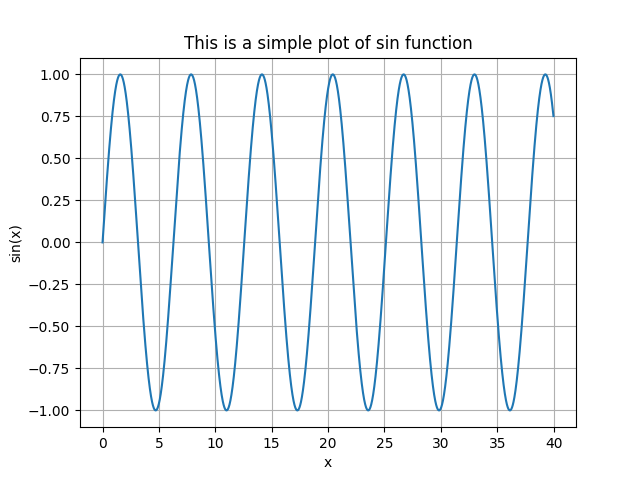
\includegraphics[width=\textwidth]{images/sin}
	\caption{Example plot from Matplotlib}
	\label{fig:matplotlib}
\end{figure}

\paragraph{}
For more information regarding Matplotlib usage please consult the official documentation available under: \url{https://matplotlib.org/2.2.2/contents.html}.

\chapter{Results}
\label{chap:results}
\paragraph{}
Let us now look at the outcomes. Inputs have been grouped into buckets depending of the angle of the split in the image by a step of 45$^{\circ}$. Dropping single image of a blurred splint (8/11) from the input set resulted in very satisfying results as presented in the tables below - both for individual angles .

\begin{table}[H]
    \centering
	\begin{spacing}{1.5}    
    \begin{tabular}{|l|l|l|}
        \hline
        \cellcolor{gray} & \textbf{Output: Same} & \textbf{Output: Different} \\ [0.5ex]
        \hline\hline
        \textbf{Actual: Same} & 12 & 1 \\ [0.5ex]
        \hline
        \textbf{Actual: Different} & 0 & 177 \\ [0.5ex]
        \hline
    \end{tabular}
    \end{spacing}
    \caption{Results for angle 0$^{\circ}$}
\end{table}
            
\begin{table}[H]
    \centering
	\begin{spacing}{1.5}    
    \begin{tabular}{|l|l|l|}
        \hline
        \cellcolor{gray} & \textbf{Output: Same} & \textbf{Output: Different} \\ [0.5ex]
        \hline\hline
        \textbf{Actual: Same} & 5 & 1 \\ [0.5ex]
        \hline
        \textbf{Actual: Different} & 0 & 130 \\ [0.5ex]
        \hline
    \end{tabular}
    \end{spacing}
    \caption{Results for angle 45$^{\circ}$}
\end{table}
            
\begin{table}[H]
    \centering
	\begin{spacing}{1.5}    
    \begin{tabular}{|l|l|l|}
        \hline
        \cellcolor{gray} & \textbf{Output: Same} & \textbf{Output: Different} \\ [0.5ex]
        \hline\hline
        \textbf{Actual: Same} & 5 & 4 \\ [0.5ex]
        \hline
        \textbf{Actual: Different} & 0 & 162 \\ [0.5ex]
        \hline
    \end{tabular}
    \end{spacing}
    \caption{Results for angle 90$^{\circ}$}
\end{table}
            
\begin{table}[H]
    \centering
	\begin{spacing}{1.5}    
    \begin{tabular}{|l|l|l|}
        \hline
        \cellcolor{gray} & \textbf{Output: Same} & \textbf{Output: Different} \\ [0.5ex]
        \hline\hline
        \textbf{Actual: Same} & 8 & 1 \\ [0.5ex]
        \hline
        \textbf{Actual: Different} & 0 & 181 \\ [0.5ex]
        \hline
    \end{tabular}
    \end{spacing}
    \caption{Results for angle 135$^{\circ}$}
\end{table}
            
\begin{table}[H]
    \centering
	\begin{spacing}{1.5}    
    \begin{tabular}{|l|l|l|}
        \hline
        \cellcolor{gray} & \textbf{Output: Same} & \textbf{Output: Different} \\ [0.5ex]
        \hline\hline
        \textbf{Actual: Same} & 10 & 2 \\ [0.5ex]
        \hline
        \textbf{Actual: Different} & 0 & 264 \\ [0.5ex]
        \hline
    \end{tabular}
    \end{spacing}
    \caption{Results for angle 180$^{\circ}$}
\end{table}
            
\begin{table}[H]
    \centering
	\begin{spacing}{1.5}    
    \begin{tabular}{|l|l|l|}
        \hline
        \cellcolor{gray} & \textbf{Output: Same} & \textbf{Output: Different} \\ [0.5ex]
        \hline\hline
        \textbf{Actual: Same} & 6 & 1 \\ [0.5ex]
        \hline
        \textbf{Actual: Different} & 0 & 164 \\ [0.5ex]
        \hline
    \end{tabular}
    \end{spacing}
    \caption{Results for angle 225$^{\circ}$}
\end{table}
            
\begin{table}[H]
    \centering
	\begin{spacing}{1.5}    
    \begin{tabular}{|l|l|l|}
        \hline
        \cellcolor{gray} & \textbf{Output: Same} & \textbf{Output: Different} \\ [0.5ex]
        \hline\hline
        \textbf{Actual: Same} & 5 & 1 \\ [0.5ex]
        \hline
        \textbf{Actual: Different} & 0 & 130 \\ [0.5ex]
        \hline
    \end{tabular}
    \end{spacing}
    \caption{Results for angle 270$^{\circ}$}
\end{table}
            
\begin{table}[H]
    \centering
	\begin{spacing}{1.5}    
    \begin{tabular}{|l|l|l|}
        \hline
        \cellcolor{gray} & \textbf{Output: Same} & \textbf{Output: Different} \\ [0.5ex]
        \hline\hline
        \textbf{Actual: Same} & 13 & 0 \\ [0.5ex]
        \hline
        \textbf{Actual: Different} & 0 & 218 \\ [0.5ex]
        \hline
    \end{tabular}
    \end{spacing}
    \caption{Results for angle 315$^{\circ}$}
\end{table}
            
\begin{table}[H]
    \centering
	\begin{spacing}{1.5}
    \begin{tabular}{|l|l|l|}
        \hline
        \cellcolor{gray} & \textbf{Output: Same} & \textbf{Output: Different} \\ [0.5ex]
        \hline\hline
        \textbf{Actual: Same} & 64 & 11 \\ [0.5ex]
        \hline
        \textbf{Actual: Different} & 0 & 1426 \\ [0.5ex]
        \hline
    \end{tabular}
    \end{spacing}
    \caption{Aggregated results}
\end{table}
        
\begin{table}[H]
    \centering
	\begin{spacing}{1.5}    
    \begin{tabular}{|l|l|l|}
        \hline
        Sensitivity                 & 0.8533333333333334 \\
        \hline
        Specificity                 & 1.0 \\
        \hline
        Positive predictive value   & 1.0 \\
        \hline
        Negative predictive value   & 0.9923451635351427 \\
        \hline
        False positive rate         & 0.0 \\
        \hline
        False negative rate         & 0.1466666666666666 \\
        \hline
        False discovery rate        & 0.0 \\
        \hline
        Accuracy                    & 0.9926715522984677 \\
        \hline
        F1 score                    & 0.920863309352518 \\
        \hline
    \end{tabular}
    \end{spacing}
    \caption{Statistical measures of the algorithm - bucketized}
\end{table}

\todo{Describe situation for all of the inputs}

\begin{table}[H]
    \centering
    \begin{spacing}{1.5}
    \begin{tabular}{|l|l|l|}
        \hline
        \cellcolor{gray} & \textbf{Output: Same} & \textbf{Output: Different} \\ [0.5ex]
        \hline\hline
        \textbf{Actual: Same} & 300 & 572 \\ [0.5ex]
        \hline
        \textbf{Actual: Different} & 5 & 11684 \\ [0.5ex]
        \hline
    \end{tabular}
    \end{spacing}
    \caption{Overall results}
\end{table}
        
\begin{table}[H]
    \centering
    \begin{spacing}{1.5}
    \begin{tabular}{|l|l|l|}
        \hline
        Sensitivity                 & 0.3440366972477064 \\
        \hline
        Specificity                 & 0.9995722474120968 \\
        \hline
        Positive predictive value   & 0.9836065573770492 \\
        \hline
        Negative predictive value   & 0.9533289817232375 \\
        \hline
        False positive rate         & 0.00042775258790317405 \\
        \hline
        False negative rate         & 0.6559633027522935 \\
        \hline
        False discovery rate        & 0.016393442622950838 \\
        \hline
        Accuracy                    & 0.9540641668656954 \\
        \hline
        F1 score                    & 0.5097706032285472 \\
        \hline
    \end{tabular}
    \end{spacing}
    \caption{Statistical measures of the algorithm - all data}
\end{table}

\todo{Add statistical tests verifyin the hypothesis that angle is important}

\chapter{Summary}
\paragraph{}
The goal of this thesis was to use image processing techniques for identification of foundry details. An algorithm has been created for comparing images of splints and detecting whether two of them represent the same object or two different objects. Despite having the images taken by a smartphone with varying lighting conditions, a satisfactory result has been achieved. Some hints for possible solutions were also provided for the preprocessing phase. The thesis presents ideas for improvements that should be considered before production implementation.

\paragraph{}
Plentitude of runs, adjustments and configurations of the algorithm over the input data has led to a hypothesis that significantly better accuracy can be achieved when the object are placed on the images under the same angle. This hypothesis has been later confirmed with results and statistical tests in chapter \ref{chap:results}.

\paragraph{}
Further on, the thesis has also provided an overview of many image processing aspects and transformations heavily used within the developed algorithm. Both the theory and also some examples were presented. All described algorithms are also available in the OpenCV library that served as the fundamental library for implementing the algorithm of splints comparison.

\paragraph{}
Last but not least, the usage of OpenCV - described before; NumPy and Matplotlib - the Python libraries also extensively used, was provided with some simple code samples that can be used as a quick starters.

\bibliographystyle{plain}
\bibliography{bibliography}

\end{document}
